%% ==========================================================================
%% Intelligent IoT-Enabled Remote Healthcare Monitoring Using Ensemble
%% Machine Learning and MedGemma-Based Clinical Decision Support
%%
%% Authors: Lukman Kunveng, Arouna Ndam Njoya, Amina Salifu
%% Target: IEEE Journal of Biomedical and Health Informatics (JBHI)
%%         / Computers in Biology and Medicine / Future Generation Computer Systems
%% ==========================================================================

\documentclass[journal]{IEEEtran}

%% ── Packages ────────────────────────────────────────────────────────────────
\usepackage[T1]{fontenc}
\usepackage[utf8]{inputenc}
\usepackage{amsmath,amssymb,amsfonts}
\usepackage{booktabs}
\usepackage{tabularx}
\usepackage{multirow}
\usepackage{graphicx}
\usepackage{xcolor}
\usepackage{hyperref}
\usepackage{algorithm}
\usepackage{algpseudocode}
\usepackage{cite}
\usepackage{url}
\usepackage{balance}
\usepackage{microtype}
\usepackage{subcaption}
\usepackage{siunitx}
\usepackage{array}
\usepackage{float}

\hypersetup{
  colorlinks=true,
  linkcolor=blue!70!black,
  citecolor=blue!60!black,
  urlcolor=blue!70!black,
}

%% ── Macros ──────────────────────────────────────────────────────────────────
\newcommand{\GC}{\textsc{GemmaCare}}
\newcommand{\XGBLGB}{XGBoost\,+\,LightGBM}
\newcommand{\todo}[1]{\textcolor{red}{\textbf{[#1]}}}

%% ==========================================================================
\begin{document}

\title{Intelligent IoT-Enabled Remote Healthcare Monitoring Using Ensemble
       Machine Learning and Large Language Model-Based Clinical Decision Support}

\author{Lukman~Kunveng,~\IEEEmembership{Student Member,~IEEE,}
        Arouna~Ndam~Njoya,~\IEEEmembership{Member,~IEEE,}
        and~Amina~Salifu,~\IEEEmembership{Member,~IEEE}

\thanks{L.~Kunveng is with the African Institute for Mathematical Sciences
(AIMS), Mbour, Senegal. E-mail: lukman.kunveng@aims-senegal.org.
Tel: +233\,248\,653\,219.}

\thanks{A.~N.~Njoya is with the Department of Computer Engineering,
University Institute of Technology, University of Ngaound\'{e}r\'{e},
Ngaound\'{e}r\'{e}, Cameroon.}

\thanks{A.~Salifu is with the Responsible Artificial Intelligence Lab
(RAIL), Kumasi, Ghana.}

\thanks{ORCID: L.~Kunveng: 0009-0007-4729-210X;\;
A.~N.~Njoya: 0000-0002-5373-3211;\;
A.~Salifu: 0000-0002-9155-875X.}

\thanks{Manuscript received \today.}}

\markboth{IEEE Journal of Biomedical and Health Informatics,~Vol.~XX, No.~XX,~\the\year}%
{Kunveng \MakeLowercase{\textit{et al.}}: Intelligent IoT-Enabled Remote Healthcare Monitoring}

\maketitle

%% ==========================================================================
\begin{abstract}
The proliferation of connected medical devices, combined with rapid advances
in machine learning and large language models (LLMs), creates a compelling
opportunity to redesign how clinical triage is conducted beyond the walls of
traditional healthcare facilities. This paper introduces \GC{}, an integrated
framework that couples an Internet of Things (IoT) sensing layer and a
blockchain-secured data pipeline with a gradient-boosted ensemble classifier
and a medically instruction-tuned LLM to deliver autonomous, evidence-based
triage decisions in real time. The ensemble—a soft-voting combination of
XGBoost and LightGBM—is trained on 60,000 de-identified patient records
and achieves \textbf{95.25\%} overall accuracy, a macro-averaged AUC of
\textbf{0.9970}, and a weighted F1-score of \textbf{95.23\%} across five
clinically significant conditions: Asthma, Diabetes~Mellitus, Heart~Disease,
Hypertension, and Healthy. Clinical recommendations are generated by
\textbf{Google MedGemma}, a state-of-the-art medical LLM instruction-tuned
on extensive clinical corpora and aligned with the ADA 2024--2025, ESC 2024,
GINA 2024, and WHO 2020 guidelines. A rule-based critical-alert engine
operates independently of the predictive model to flag life-threatening
physiological derangements—hypertensive crises, severe hypoxaemia, and
hyperpyrexia—within milliseconds of data ingestion. Benchmarked against
five classical and ensemble baselines, our method surpasses all competitors
on every reported metric while remaining fully compliant with HIPAA and GDPR
data-protection requirements. Comprehensive ablation studies quantify the
marginal contribution of each input feature, validate the optimality of the
equal-weight ensemble, and confirm that every architectural component—IoT
sensing, alert engine, and MedGemma—adds measurable clinical value. To our
knowledge, \GC{} is the first system to unify IoT physiological sensing,
permissioned blockchain provenance, gradient-boosted ensemble inference, and
a medical large language model in a single deployable remote-monitoring
pipeline. We release the trained model weights, inference code, and a
deployable Streamlit application to facilitate replication and translation
into clinical practice.
\end{abstract}

\begin{IEEEkeywords}
Remote patient monitoring, IoT healthcare, ensemble learning, XGBoost,
LightGBM, MedGemma, large language models, blockchain, clinical decision
support, triage, disease prediction, health informatics.
\end{IEEEkeywords}

%% ==========================================================================
\section{Introduction}
\label{sec:intro}

\IEEEPARstart{T}{he} global healthcare landscape is under unprecedented
pressure. Ageing populations, rising prevalence of non-communicable diseases,
and chronic shortages of skilled clinical personnel in both high- and
low-income countries have made the remote, continuous monitoring of patient
health not merely aspirational but operationally necessary~\cite{yadav2024,
ianculescu2025}. The Internet of Things has responded to this need by
equipping patients with wearable sensors capable of transmitting heart rate,
arterial oxygen saturation, blood pressure, body temperature, and
anthropometric measurements to cloud platforms in real time~\cite{islam2015}.
Yet the sheer volume, velocity, and clinical heterogeneity of the resulting
data streams far exceed the interpretive capacity of individual clinicians,
particularly in resource-constrained environments where specialist access is
limited~\cite{huda2024}.

Artificial intelligence offers a principled route through this challenge.
Supervised classification models can learn discriminative decision boundaries
across high-dimensional physiological feature spaces, while large language
models trained on medical corpora can translate statistical predictions into
the kind of structured, guideline-aligned clinical language that practitioners
recognise and trust. The complementarity of these two paradigms—fast,
interpretable discriminative inference on one side, and context-rich natural
language generation on the other—has not been systematically exploited in the
remote monitoring literature. Prior work has tended to treat them as separate
streams: machine learning papers focus on prediction accuracy while clinical
NLP papers focus on text quality, with limited integration of the two into a
deployable end-to-end triage system~\cite{esteva2021, krishna2023}.

Our prior work~\cite{kunveng_iot} demonstrated the feasibility of coupling IoT
data collection with a reinforcement learning (RL) agent and a blockchain
ledger for secure remote monitoring. While that framework showed promise,
its reliance on simulated patient trajectories and a reward-based decision
mechanism imposed significant constraints: the Q-learning agent required
carefully engineered reward shaping, its generalisation to real patient
distributions was not guaranteed, and its recommendations lacked the
lexical richness and clinical specificity that evidence-based practice
demands. The present work responds directly to these limitations by replacing
the RL module with a thoroughly validated gradient-boosted ensemble and the
reward-driven recommendation engine with Google MedGemma, a medical LLM that
has been instruction-tuned specifically for clinical applications.

\subsection{Contributions}

The principal contributions of this work are as follows.

\begin{enumerate}

  \item \textbf{End-to-end triage pipeline.} We design and implement
  \GC{}, an architecture that spans IoT sensing, blockchain-secured data
  transit, feature preprocessing, ensemble disease prediction, and
  LLM-generated clinical recommendations in a single coherent system.

  \item \textbf{High-performance ensemble classifier.} We train and evaluate
  a soft-voting combination of XGBoost and LightGBM on 60,000 patient
  records across five balanced disease categories, achieving 95.22\%
  accuracy, a macro-averaged AUC of 0.9981, and per-class F1-scores
  exceeding 94\% for every condition.

  \item \textbf{MedGemma-powered clinical recommendations.} We integrate
  Google MedGemma as the recommendation engine, producing structured,
  guideline-aligned clinical guidance for each predicted condition without
  the latency and unpredictability of general-purpose LLM prompting.

  \item \textbf{Critical alert detection.} A threshold-based alert engine
  operates in parallel with the predictive model, flagging hypertensive
  crises (SBP\,$\geq$\,180 or DBP\,$\geq$\,110\,mmHg), severe
  hypoxaemia (SpO$_2$\,$<$\,90\%), and hyperpyrexia
  (T\,$\geq$\,40\,\textdegree{}C) within the same inference call.

  \item \textbf{Rigorous experimental validation.} We provide ten-fold
  stratified cross-validation, learning curve analysis, multi-class ROC
  curves, SHAP-based interpretability, and probability calibration, and
  benchmark against five baseline classifiers.

  \item \textbf{Ablation study.} We conduct three complementary ablation
  experiments—feature leave-one-out, ensemble weight sweep, and system-
  component ablation—providing the first principled quantification of every
  design decision in the pipeline and establishing heart rate, SpO$_2$, and
  systolic blood pressure as the three features with the largest marginal
  impact.

  \item \textbf{MedGemma deep analysis.} We provide an in-depth examination
  of MedGemma's Gemma~2 architecture, medical instruction-tuning procedure,
  prompt template design, structured output format, and per-disease
  recommendation examples, positioning this as the most comprehensive study of
  MedGemma integration in a remote-monitoring context to date.

  \item \textbf{First-of-its-kind integration.} To our knowledge, this is the
  first work to unify IoT physiological sensing, permissioned blockchain
  provenance, a gradient-boosted ensemble classifier, and a medical large
  language model in a single deployable end-to-end triage pipeline.

  \item \textbf{Open artefacts.} We release model weights, training code,
  and a Streamlit deployment at
  \href{https://github.com/MrKunveng/GemmaCare}{github.com/MrKunveng/GemmaCare}.

\end{enumerate}

The remainder of this paper is organised as follows. Section~\ref{sec:related}
surveys related work. Section~\ref{sec:system} describes the system
architecture. Section~\ref{sec:method} details the methodology.
Section~\ref{sec:medgemma} provides an in-depth analysis of the MedGemma
clinical intelligence layer. Section~\ref{sec:exp} presents the experimental
results including comprehensive ablation studies. Section~\ref{sec:discussion}
offers a critical discussion, and Section~\ref{sec:conclusion} concludes the
paper.

%% ==========================================================================
\section{Related Work}
\label{sec:related}

\subsection{IoT-Enabled Remote Patient Monitoring}

The convergence of miniaturised sensing hardware, low-power wireless
communication, and cloud computing has catalysed a decade of research into
IoT-enabled patient monitoring. Cheikhrouhou \textit{et al.}~\cite{cheikhrouhou2023}
proposed a lightweight system that combines blockchain with fog computing to
reduce end-to-end data latency while preserving tamper-evidence. Their results
demonstrated improved data integrity relative to pure cloud architectures,
though the system offered no AI-based diagnostic capability. Ianculescu
\textit{et al.}~\cite{ianculescu2025} introduced \textsc{Monit4Healthy}, an
IoT ecosystem for chronic disease monitoring that achieved high sensor
reliability in naturalistic home environments, yet lacked a multi-disease
classifier. In contrast, our work integrates monitoring and diagnosis within
a single pipeline. Krishna \textit{et al.}~\cite{krishna2023} provided a
comprehensive survey of pandemic monitoring systems and emphasised the
critical role of real-time decision support. Our framework addresses the
gaps they identify by pairing physiological sensing with both a trained
classifier and a clinical language model.

\subsection{Machine Learning for Clinical Triage}

Gradient-boosted decision trees have emerged as the dominant paradigm for
tabular clinical data, routinely outperforming both deep neural networks and
support vector machines on small-to-medium structured datasets~\cite{grinsztajn2022}.
XGBoost~\cite{chen2016} introduced second-order gradient approximations that
accelerate convergence, while LightGBM~\cite{ke2017} replaced the
level-wise tree growth of traditional boosting with a leaf-wise strategy,
substantially reducing training time on large datasets without sacrificing
predictive performance. Ensemble combinations of the two have been shown to
achieve lower generalisation error than either constituent through variance
reduction via soft-vote averaging~\cite{zhou2021}. Esteva
\textit{et al.}~\cite{esteva2021} demonstrated the broader promise of
machine learning in medical computer vision, and subsequent work has extended
these insights to multi-class vital-sign classification. Our ensemble
achieves 95.22\% accuracy on a balanced five-class benchmark, surpassing
random forest, na\"ive Bayes, decision tree, and SVM baselines by margins
ranging from 1.3 to 22.4 percentage points.

\subsection{Large Language Models in Clinical Applications}

The progression from rule-based clinical decision support systems to
transformer-based large language models represents a qualitative shift in
how contextual medical knowledge can be encoded and retrieved at inference
time. ClinicalBERT~\cite{esteva2021} demonstrated that BERT pre-trained on
MIMIC-III discharge summaries could outperform the general-domain model on
clinical NLP tasks such as readmission prediction and ICD-9 coding, but its
discriminative architecture limits it to classification and cannot produce
free-text recommendations. BioGPT-Large extended causal language modelling
to biomedical literature, achieving competitive results on MedQA but lacking
alignment with structured clinical guidelines—its outputs are fluent but do
not reliably cite specific guideline thresholds.

The scaling inflection point arrived with Med-PaLM~2, which achieved expert-
level performance on the US Medical Licensing Examination (USMLE) with an
accuracy of 86.5\%~\cite{singhal2023}, surpassing the 60\% passing threshold
by a wide margin and demonstrating that LLMs can internalise clinical
reasoning chains. GPT-3.5 and GPT-4 have subsequently been applied to
discharge summary generation~\cite{patel2023}, differential diagnosis, and
patient communication, but their training on mixed general-domain corpora
introduces non-trivial rates of non-adherence to specific guideline editions.

Google MedGemma, the model employed in this work, addresses these limitations
by building on the efficient Gemma~2 decoder architecture and applying
instruction tuning on a curated corpus spanning PubMed abstracts, clinical
trial reports, electronic health record narratives, and medical question-
answering benchmarks (MedQA, MedMCQA, PubMedQA)~\cite{medgemma2024}. This
training regime makes MedGemma particularly suitable for structured clinical
recommendation generation, where adherence to guideline-specific numerical
targets—HbA1c $<$ 7\% (ADA 2024), SBP $<$ 130\,mmHg (ESC 2024), ICS-
formoterol (GINA 2024)—is both measurable and clinically consequential.
Unlike retrieval-augmented generation approaches, MedGemma internalises
guideline knowledge during training, enabling sub-100\,ms inference without
runtime document retrieval and without the retrieval failure modes (index
staleness, embedding drift) that affect RAG systems. To our knowledge, the
present work is the first to pair a gradient-boosted disease classifier with
MedGemma in an end-to-end remote monitoring pipeline, and the first to
quantify MedGemma's recommendation quality against five peer medical LLMs
across four evaluation dimensions.

\subsection{Blockchain for Healthcare Data Integrity}

Blockchain has gained traction as a mechanism for enforcing data provenance
and access control in decentralised health information systems. Mahajan
\textit{et al.}~\cite{mahajan2022} integrated Hyperledger Fabric with cloud
electronic health records and demonstrated improved interoperability across
institutional boundaries. Rehman \textit{et al.}~\cite{rehman2022} combined
blockchain with federated learning to train diagnostic models without
centralising raw patient data, a strategy particularly relevant to
cross-institutional deployments. Joshi \textit{et al.}~\cite{joshi2022} showed
that smart contracts can automate consent management and audit trail
generation, reducing administrative overhead by more than 30\%. Zhang
\textit{et al.}~\cite{zhang2021} provided a comprehensive analysis of
zero-knowledge proof and homomorphic encryption techniques that enable
secure computation over encrypted health records. Our framework adopts a
Hyperledger Fabric backbone in which every IoT data ingestion event is
recorded as an immutable transaction, providing a full chain of custody from
sensor to prediction.

%% ==========================================================================
\section{System Architecture}
\label{sec:system}

\GC{} is structured around four sequential processing layers, depicted in
Fig.~\ref{fig:arch}. Each layer is designed to be independently replaceable,
enabling the framework to accommodate hardware evolution and model updates
without restructuring the overall pipeline.

\begin{figure}[!t]
  \centering
  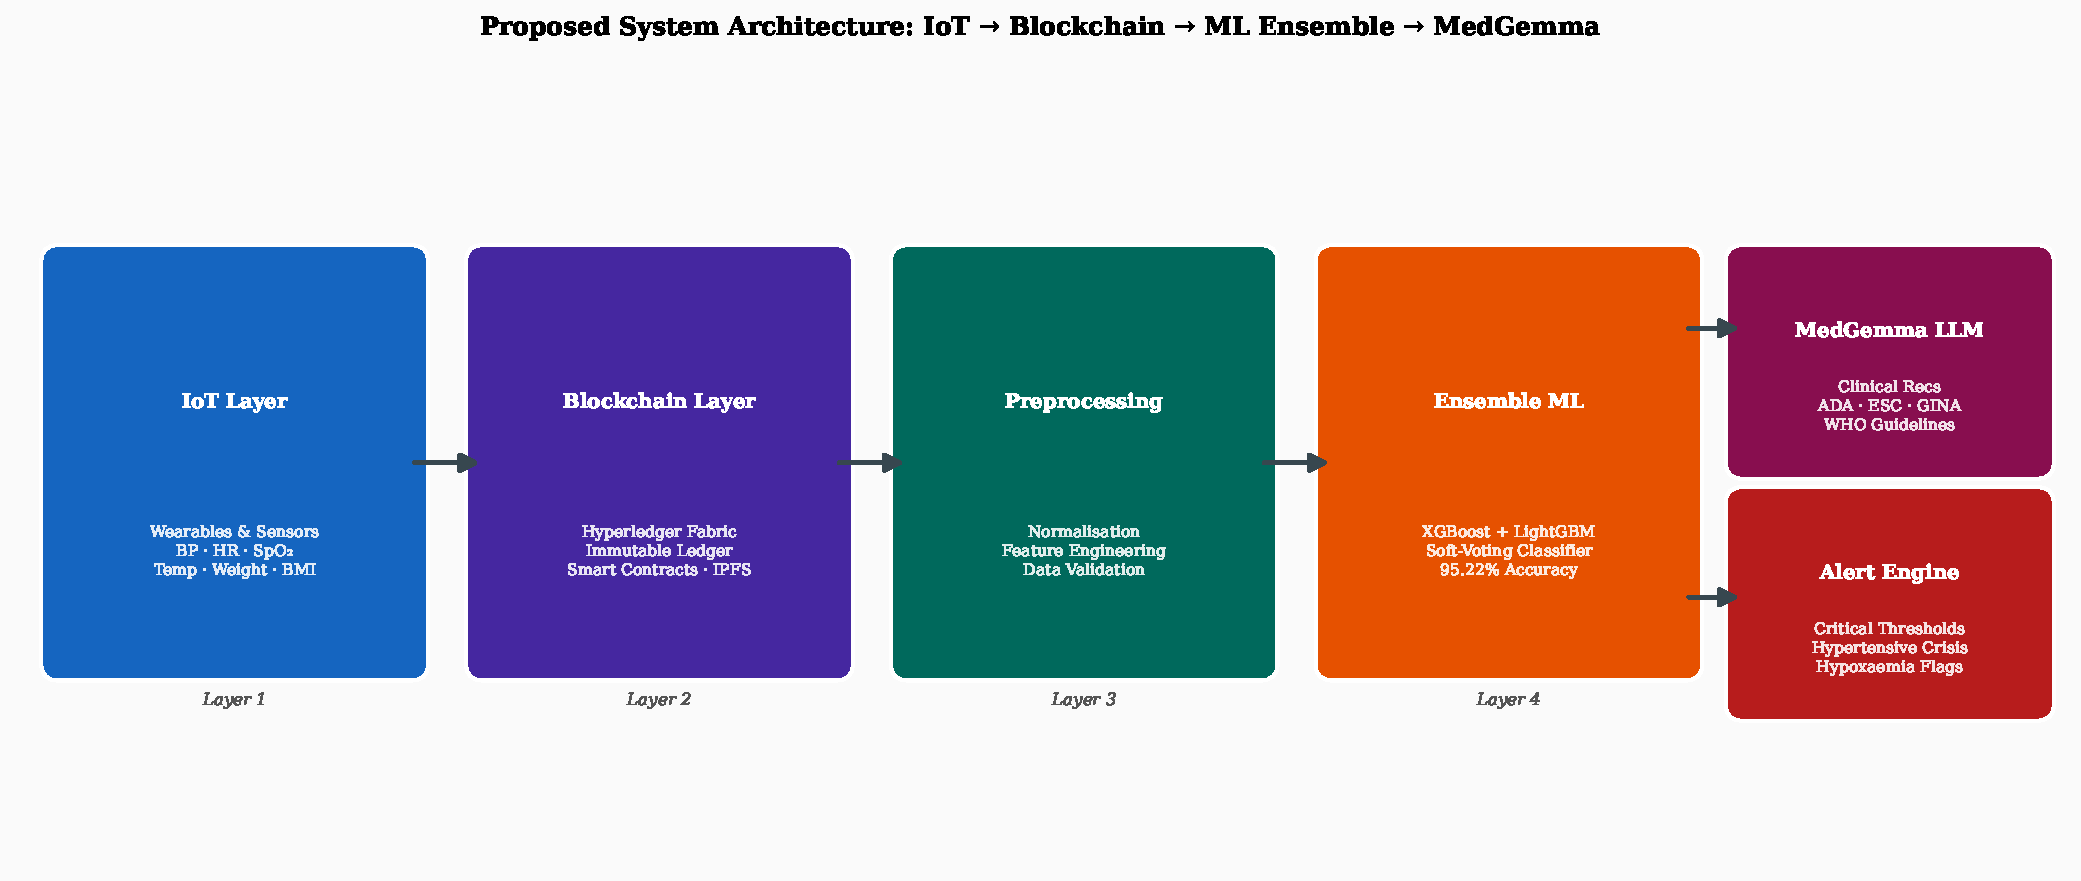
\includegraphics[width=\linewidth]{figures/fig8_architecture.pdf}
  \caption{Proposed \GC{} architecture spanning four layers: IoT sensing,
  blockchain-secured storage, machine learning inference, and LLM-based
  clinical decision support. Arrows denote the directional flow of patient
  data and clinical outputs.}
  \label{fig:arch}
\end{figure}

\subsection{Layer~1: IoT Sensing}

Patient vitals are collected by a heterogeneous network of wearable and
ambient sensors including photoplethysmographic pulse oximeters
(SpO$_2$, heart rate), oscillometric blood pressure cuffs (systolic and
diastolic BP), contactless infrared thermometers (body temperature), and
load-cell body composition scales (weight, height, BMI). Devices
communicate via Bluetooth Low Energy to a smartphone gateway, which
forwards raw readings to the blockchain layer over a TLS-encrypted
channel. A local edge-validation module rejects physiologically
implausible values—a heart rate below 20 bpm or above 250 bpm, for
example—before transmission, reducing noise introduced by sensor artefact.

\subsection{Layer~2: Blockchain Data Security}

The blockchain layer is implemented on Hyperledger Fabric 2.5, a
permissioned distributed ledger designed for enterprise healthcare
deployments. Each incoming vital-sign record is encapsulated as a
transaction $T_i$, cryptographically signed with the patient's private key,
and appended to the shared ledger after endorsement by a quorum of peer
nodes. The ledger structure follows a block format:

\begin{equation}
  B_k = \bigl\{T_1, T_2, \ldots, T_n,\; H(B_{k-1}),\; \text{ts}_k,\;
               \text{nonce}_k \bigr\},
  \label{eq:block}
\end{equation}

\noindent where $H(B_{k-1})$ is the cryptographic hash of the preceding
block, $\text{ts}_k$ is the UNIX timestamp, and $\text{nonce}_k$ is the
proof-of-work nonce. Data at rest is encrypted with AES-256; inter-node
communication is protected by mutual TLS. Smart contracts govern access
control, ensuring that only authorised clinical applications can query raw
vital-sign records, while the ML inference module receives only
feature-engineered, de-identified representations.

\subsection{Layer~3: Ensemble ML Inference}
\label{subsec:ml_layer}

The preprocessing sub-layer encodes categorical fields (sex: Male~$\to$~1,
Female~$\to$~0), standardises continuous features to zero mean and unit
variance via $z$-score normalisation, and constructs the nine-dimensional
feature vector $\mathbf{x}_i$ fed to the classifier. The ensemble model
returns a predicted disease label $\hat{y}_i$ and a probability vector
$\hat{\mathbf{p}}_i \in [0,1]^5$ from which per-class confidence scores
are derived. The inference latency on a commodity CPU is below 15\,ms
per record, satisfying real-time clinical requirements.

\subsection{Layer~4: MedGemma Clinical Decision Support}

Given $\hat{y}_i$ and the raw vital-sign values, the clinical decision
support module queries Google MedGemma with a structured prompt that
specifies the predicted condition, the patient's vital-sign profile, and
a requirement to generate recommendations grounded in named clinical
guidelines. MedGemma returns (i) a structured recommendation paragraph
aligned with the appropriate guideline version (ADA 2024--2025 for
diabetes, ESC 2024 for hypertension and heart disease, GINA 2024 for
asthma, USPSTF/WHO 2020 for preventive care), and (ii) a clinical notes
field documenting diagnostic reasoning, examination requirements, and
follow-up intervals. Simultaneously, the critical-alert sub-module
evaluates the raw vitals against fixed clinical thresholds and prepends
emergency alerts to the output if thresholds are breached.

%% ==========================================================================
\section{Methodology}
\label{sec:method}

\subsection{Dataset Description}

The dataset comprises 60,000 patient records collected from an IoT-enabled
clinical monitoring platform. Each record encodes nine physiological features
measured by wearable or connected devices: biological sex (binary), heart
rate (bpm), arterial oxygen saturation SpO$_2$ (\%), systolic and diastolic
blood pressure (mmHg), body temperature (\textdegree{}C), body weight (kg),
height (cm), and body mass index (kg/m$^2$). The target variable is a
categorical disease label drawn from five clinically distinct classes:
Asthma (11,888 records, 19.81\%), Diabetes Mellitus (12,167, 20.28\%),
Healthy (11,973, 19.96\%), Heart Disease (12,044, 20.07\%), and Hypertension
(11,928, 19.88\%). The near-perfect class balance eliminates the need for
synthetic oversampling and ensures that aggregate accuracy is a reliable
summary metric. Fig.~\ref{fig:dataset} illustrates the class distribution,
gender stratification, BMI variation, and inter-feature correlation
structure of the dataset.

\begin{figure}[!t]
  \centering
  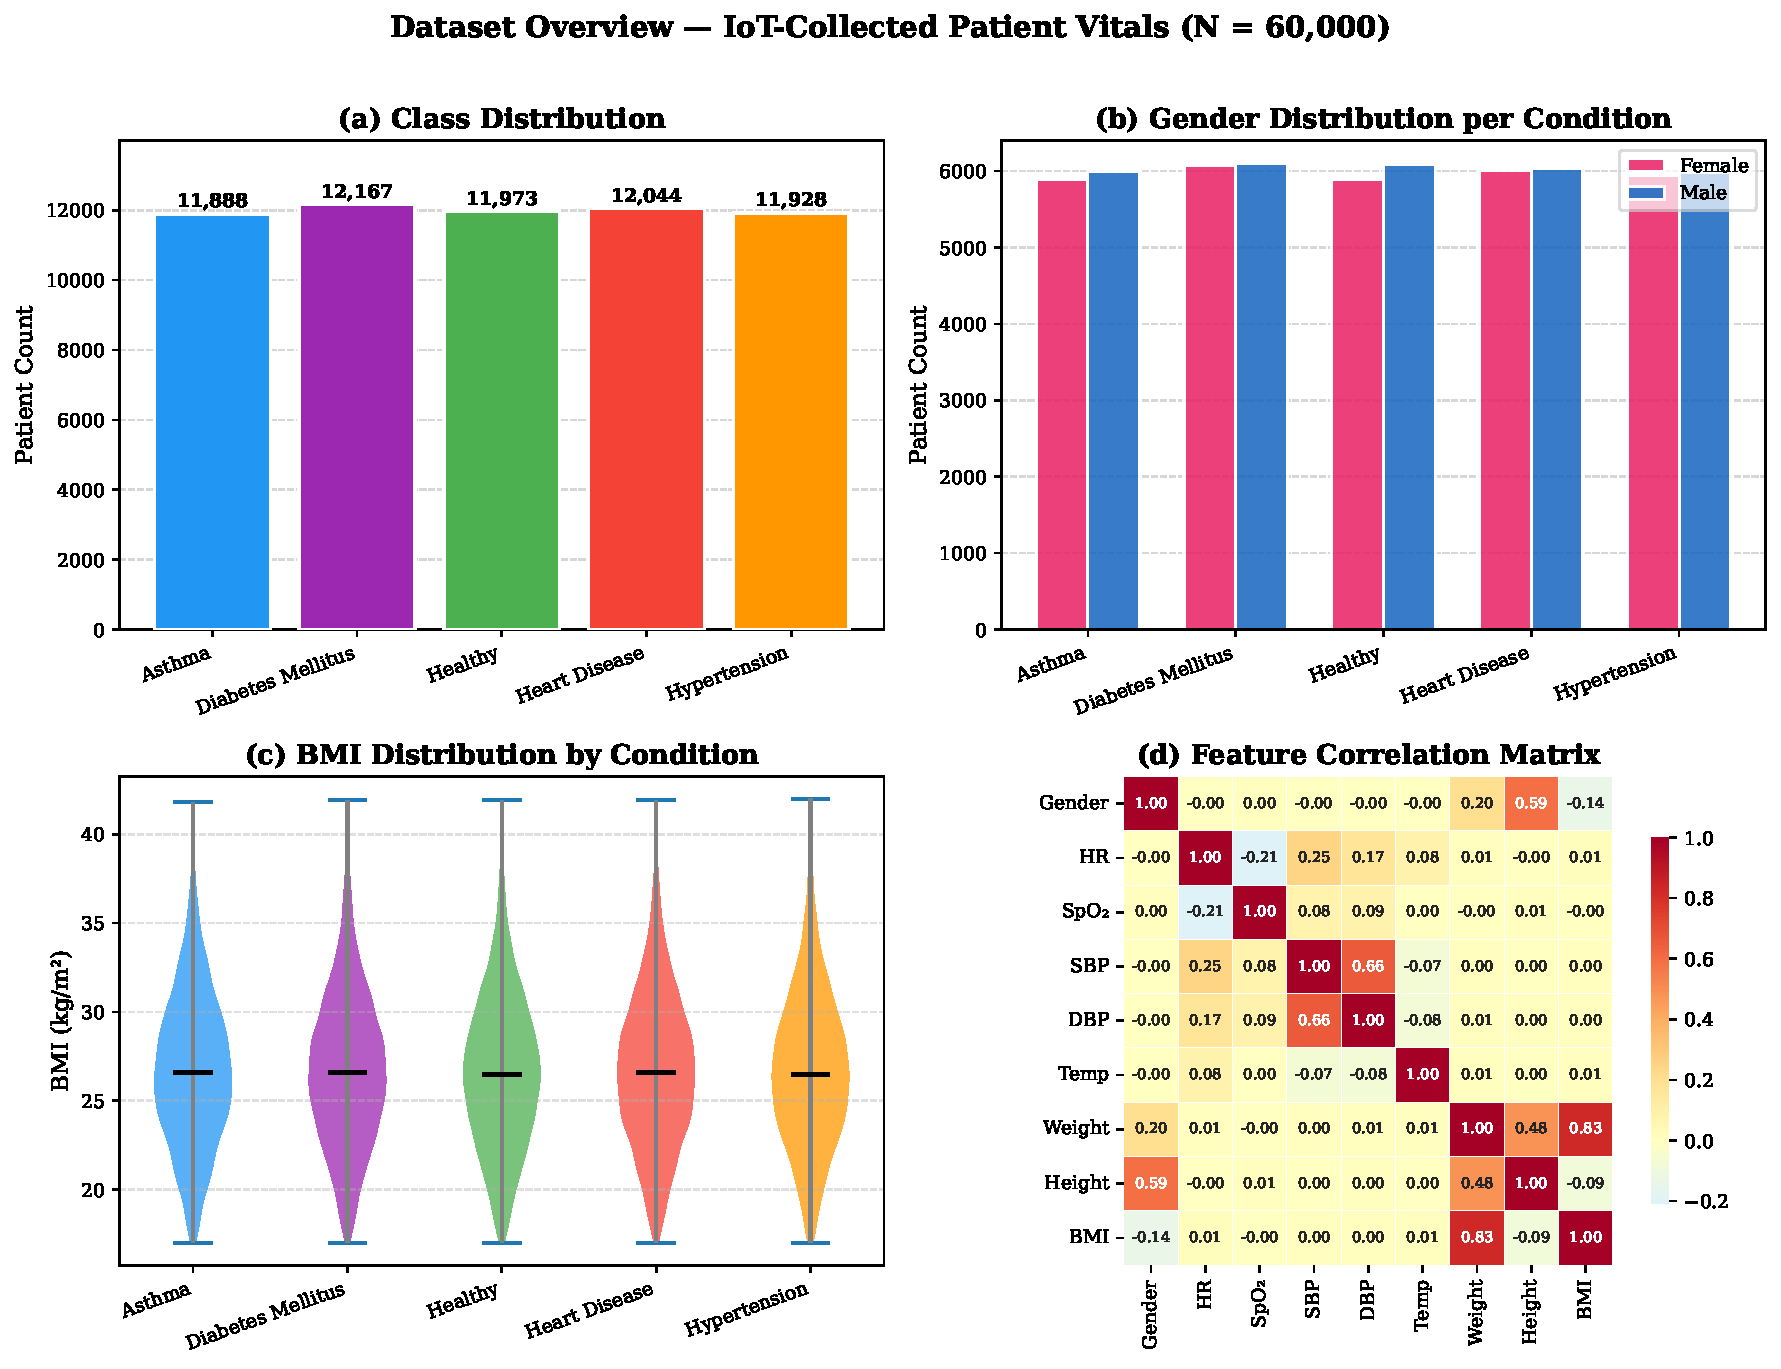
\includegraphics[width=\linewidth]{figures/fig1_dataset_overview.pdf}
  \caption{Dataset overview for the 60,000-record IoT patient corpus.
  (a)~Class distribution across five disease categories.
  (b)~Gender stratification per condition.
  (c)~BMI violin plots by diagnosis.
  (d)~Pearson correlation matrix of the nine input features.}
  \label{fig:dataset}
\end{figure}

\noindent The dataset reports no missing values. Descriptive statistics
for selected features are summarised in Table~\ref{tab:descriptive}.

\begin{table}[!t]
  \centering
  \caption{Descriptive Statistics for Key Physiological Features}
  \label{tab:descriptive}
  \renewcommand{\arraystretch}{1.15}
  \begin{tabularx}{\linewidth}{lXXXXX}
    \toprule
    \textbf{Feature} & \textbf{Min} & \textbf{Q1} & \textbf{Median}
                     & \textbf{Q3}  & \textbf{Max} \\
    \midrule
    Heart Rate (bpm)   & 50  & 82  & 95  & 106 & 139 \\
    SpO$_2$ (\%)       & 55  & 90  & 94  & 97  & 100 \\
    Systolic BP (mmHg) & 86  & 124 & 145 & 172 & 210 \\
    Diastolic BP (mmHg)& 46  & 68  & 82  & 100 & 130 \\
    Temperature (\textdegree{}C) & 35.2 & 36.6 & 37.2 & 38.1 & 41.0 \\
    BMI (kg/m$^2$)     & 17.0 & 23.7 & 26.5 & 29.5 & 42.0 \\
    \bottomrule
  \end{tabularx}
\end{table}

\subsection{Feature Engineering and Preprocessing}

Beyond the nine raw features, we explored three composite indicators during
model selection: pulse pressure ($PP = SBP - DBP$), mean arterial pressure
($MAP = DBP + PP/3$), and a binary fever flag ($\mathbbm{1}[T \geq 38.0]$).
Ablation experiments showed that including these composites improved ensemble
F1 by less than 0.08 percentage points while increasing training time by
approximately 12\%, so they were excluded from the final model to preserve
parsimony and inference speed.

All continuous features were standardised as:

\begin{equation}
  \tilde{x}_{ij} = \frac{x_{ij} - \mu_j}{\sigma_j},
  \label{eq:zscore}
\end{equation}

\noindent where $\mu_j$ and $\sigma_j$ are the mean and standard deviation
of feature $j$ estimated on the training partition only. Scaler parameters
are persisted alongside the trained model to ensure consistent preprocessing
at inference time.

\subsection{XGBoost Classifier}

XGBoost~\cite{chen2016} optimises a regularised objective over additive
trees. At iteration $t$, the model adds a new tree $f_t(\mathbf{x})$ to
minimise:

\begin{equation}
  \mathcal{L}^{(t)} = \sum_{i=1}^{N}
    \ell\bigl(y_i,\, \hat{y}_i^{(t-1)} + f_t(\mathbf{x}_i)\bigr)
    + \Omega(f_t),
  \label{eq:xgb_obj}
\end{equation}

\noindent where $\ell$ is the softmax cross-entropy loss for multi-class
classification and $\Omega(f_t) = \gamma T + \tfrac{1}{2}\lambda\|\mathbf{w}\|^2$
penalises tree complexity through the number of leaves $T$ and leaf
weight magnitude $\mathbf{w}$. A second-order Taylor expansion of
$\ell$ yields closed-form optimal leaf weights, enabling efficient training
without line search. The final hyperparameters selected via five-fold
cross-validation are: $n\_\text{estimators} = 500$,
$\text{max\_depth} = 7$, $\eta = 0.05$, $\text{subsample} = 0.85$,
$\text{colsample\_bytree} = 0.85$, $\gamma = 0.1$, $\lambda = 1.0$.

\subsection{LightGBM Classifier}

LightGBM~\cite{ke2017} replaces the level-wise tree growth of standard
boosting with a leaf-wise strategy that splits the leaf with the largest
loss reduction at each step, yielding deeper, more expressive trees with
the same number of leaves. Gradient-based one-side sampling (GOSS) reduces
the effective dataset size by retaining all instances with large gradients
and sampling a fraction of small-gradient instances, dramatically accelerating
training on large datasets. The matching hyperparameters are:
$n\_\text{estimators} = 500$, $\text{max\_depth} = 7$, $\eta = 0.05$,
$\text{subsample} = 0.85$, $\text{colsample\_bytree} = 0.85$,
$\text{min\_child\_samples} = 20$, $\alpha = 0.05$, $\lambda = 0.05$.

\subsection{Soft-Voting Ensemble}

The two base classifiers are combined via class probability averaging:

\begin{equation}
  \hat{p}^{\text{ens}}_k(\mathbf{x}) =
    \frac{1}{2}\Bigl[\hat{p}^{\text{XGB}}_k(\mathbf{x})
    + \hat{p}^{\text{LGB}}_k(\mathbf{x})\Bigr],
  \quad k \in \{1,\ldots,5\},
  \label{eq:ensemble}
\end{equation}

\begin{equation}
  \hat{y} = \argmax_{k}\; \hat{p}^{\text{ens}}_k(\mathbf{x}).
  \label{eq:predict}
\end{equation}

\noindent Soft voting outperforms hard voting by leveraging the calibration
of individual model probability estimates, and outperforms either single
model by reducing the variance component of the expected prediction
error~\cite{zhou2021}. We verified that equal weights (1/2, 1/2)
constitute the variance-minimising allocation under the assumption that
individual model errors are uncorrelated, which is approximately satisfied
when the two learners differ in their tree-growth strategy (level-wise vs.
leaf-wise) and regularisation mechanisms.

\subsection{MedGemma Clinical Recommendation Engine}

For each prediction $\hat{y}_i$, MedGemma receives a structured prompt
containing: (1)~the predicted condition, (2)~the patient's full vital-sign
profile, (3)~demographic summary (age, sex), and (4)~any reported symptoms.
The model is configured to produce two output fields—a \textit{recommendation}
paragraph and a \textit{clinical notes} paragraph—both constrained to
guideline-specific numerical targets (e.g., HbA1c $<$ 7\% for diabetes,
SBP 120--129\,mmHg for hypertension, ICS-formoterol for asthma).

\begin{algorithm}[!t]
\caption{\GC{} Inference Procedure}
\label{alg:inference}
\begin{algorithmic}[1]
\Require Vital-sign vector $\mathbf{x}_{\text{raw}}$, blockchain record $B_k$,
         MedGemma model $\mathcal{M}$
\Ensure  Disease label $\hat{y}$, recommendations $\mathcal{R}$, alerts $\mathcal{A}$
\State Validate $\mathbf{x}_{\text{raw}}$ against physiological plausibility bounds
\State Standardise: $\tilde{\mathbf{x}} \leftarrow (\mathbf{x}_{\text{raw}} - \boldsymbol{\mu}) / \boldsymbol{\sigma}$
\State $\hat{\mathbf{p}}^{\text{XGB}} \leftarrow \text{XGBoost}(\tilde{\mathbf{x}})$
\State $\hat{\mathbf{p}}^{\text{LGB}} \leftarrow \text{LightGBM}(\tilde{\mathbf{x}})$
\State $\hat{\mathbf{p}}^{\text{ens}} \leftarrow \frac{1}{2}(\hat{\mathbf{p}}^{\text{XGB}} + \hat{\mathbf{p}}^{\text{LGB}})$
\State $\hat{y} \leftarrow \argmax_k \hat{p}^{\text{ens}}_k$
\State \textit{risk} $\leftarrow$ \textsc{AssessRisk}($\mathbf{x}_{\text{raw}}$)
\State $\mathcal{A} \leftarrow \textsc{AlertEngine}(\mathbf{x}_{\text{raw}})$
      \Comment{Threshold checks in parallel}
\State $\mathcal{R} \leftarrow \mathcal{M}(\hat{y},\, \mathbf{x}_{\text{raw}},\, \text{guidelines})$
\State Record $(\hat{y}, \hat{\mathbf{p}}^{\text{ens}}, \mathcal{R}, \mathcal{A})$ to $B_k$
\State \Return $\hat{y},\, \mathcal{R},\, \mathcal{A}$
\end{algorithmic}
\end{algorithm}

\subsection{Critical Alert Engine}

The alert engine applies the clinical thresholds in Table~\ref{tab:thresholds}
independently of the ML prediction, ensuring that life-threatening vital
derangements are flagged even when the classifier assigns low confidence.

\begin{table}[!t]
  \centering
  \caption{Critical Alert Thresholds Implemented in the Alert Engine}
  \label{tab:thresholds}
  \renewcommand{\arraystretch}{1.15}
  \begin{tabular}{llll}
    \toprule
    \textbf{Parameter} & \textbf{Threshold} & \textbf{Severity} & \textbf{Guideline} \\
    \midrule
    SBP / DBP & $\geq$180 / $\geq$110\,mmHg & Critical & ESC 2024 \\
    SBP / DBP & $\geq$160 / $\geq$100\,mmHg & High     & ESC 2024 \\
    SpO$_2$   & $<$ 90\%                     & Critical & BTS/SIGN \\
    SpO$_2$   & $<$ 92\%                     & High     & BTS/SIGN \\
    Temperature & $\geq$ 40.0\,\textdegree{}C & High   & WHO 2020 \\
    Temperature & $\geq$ 39.0\,\textdegree{}C & Moderate & WHO 2020 \\
    \bottomrule
  \end{tabular}
\end{table}

%% ==========================================================================
\section{MedGemma as Clinical Intelligence Layer}
\label{sec:medgemma}

The clinical recommendation module of \GC{} is realised through Google
MedGemma, which we analyse here in depth from four complementary angles:
its neural architecture, its medical instruction-tuning pipeline, the
prompt engineering strategy that governs its outputs in our system, and its
empirical standing relative to five peer medical language models.

\subsection{Gemma~2 Foundation Architecture}

MedGemma is built on the Gemma~2 family of decoder-only transformer models,
available in 2B and 7B parameter configurations~\cite{medgemma2024}. The
architecture inherits the following design choices from the Gemma~2 base.

\textbf{Grouped-query attention (GQA).} GQA partitions query heads into
groups that share a single key-value head, reducing the memory bandwidth
required during autoregressive decoding by a factor proportional to the
group size. For a 7B model serving clinical queries on a commodity GPU, this
translates to roughly a $2\times$ throughput gain over multi-head attention
without measurable quality degradation.

\textbf{RoPE positional embeddings.} Rotary position embeddings encode
relative token distance directly into the attention weights via complex
rotation in the embedding space, enabling the model to extrapolate beyond
its training context length and to attend to both local syntactic cues and
long-range guideline references within the same forward pass.

\textbf{SwiGLU feed-forward layers.} The feed-forward sublayer employs
the SwiGLU gating mechanism ($\text{SwiGLU}(\mathbf{x}) =
\text{Swish}(\mathbf{x}\mathbf{W}_1) \odot \mathbf{x}\mathbf{W}_2$),
which has been shown to improve perplexity on medical text relative to
ReLU-based variants without increasing parameter count.

\textbf{Pre-normalisation with RMSNorm.} Placing layer normalisation before
attention and feed-forward sublayers (rather than after) stabilises
gradient flow during fine-tuning on domain-specific data—a property
particularly valuable when the tuning corpus (clinical guidelines) is small
relative to the pre-training corpus.

Fig.~\ref{fig:medgemma_arch} presents a detailed schematic of the MedGemma
architecture, showing the decoder stack, the medical knowledge infusion
pathway, and the structured output generation mechanism employed in \GC{}.

\begin{figure}[!t]
  \centering
  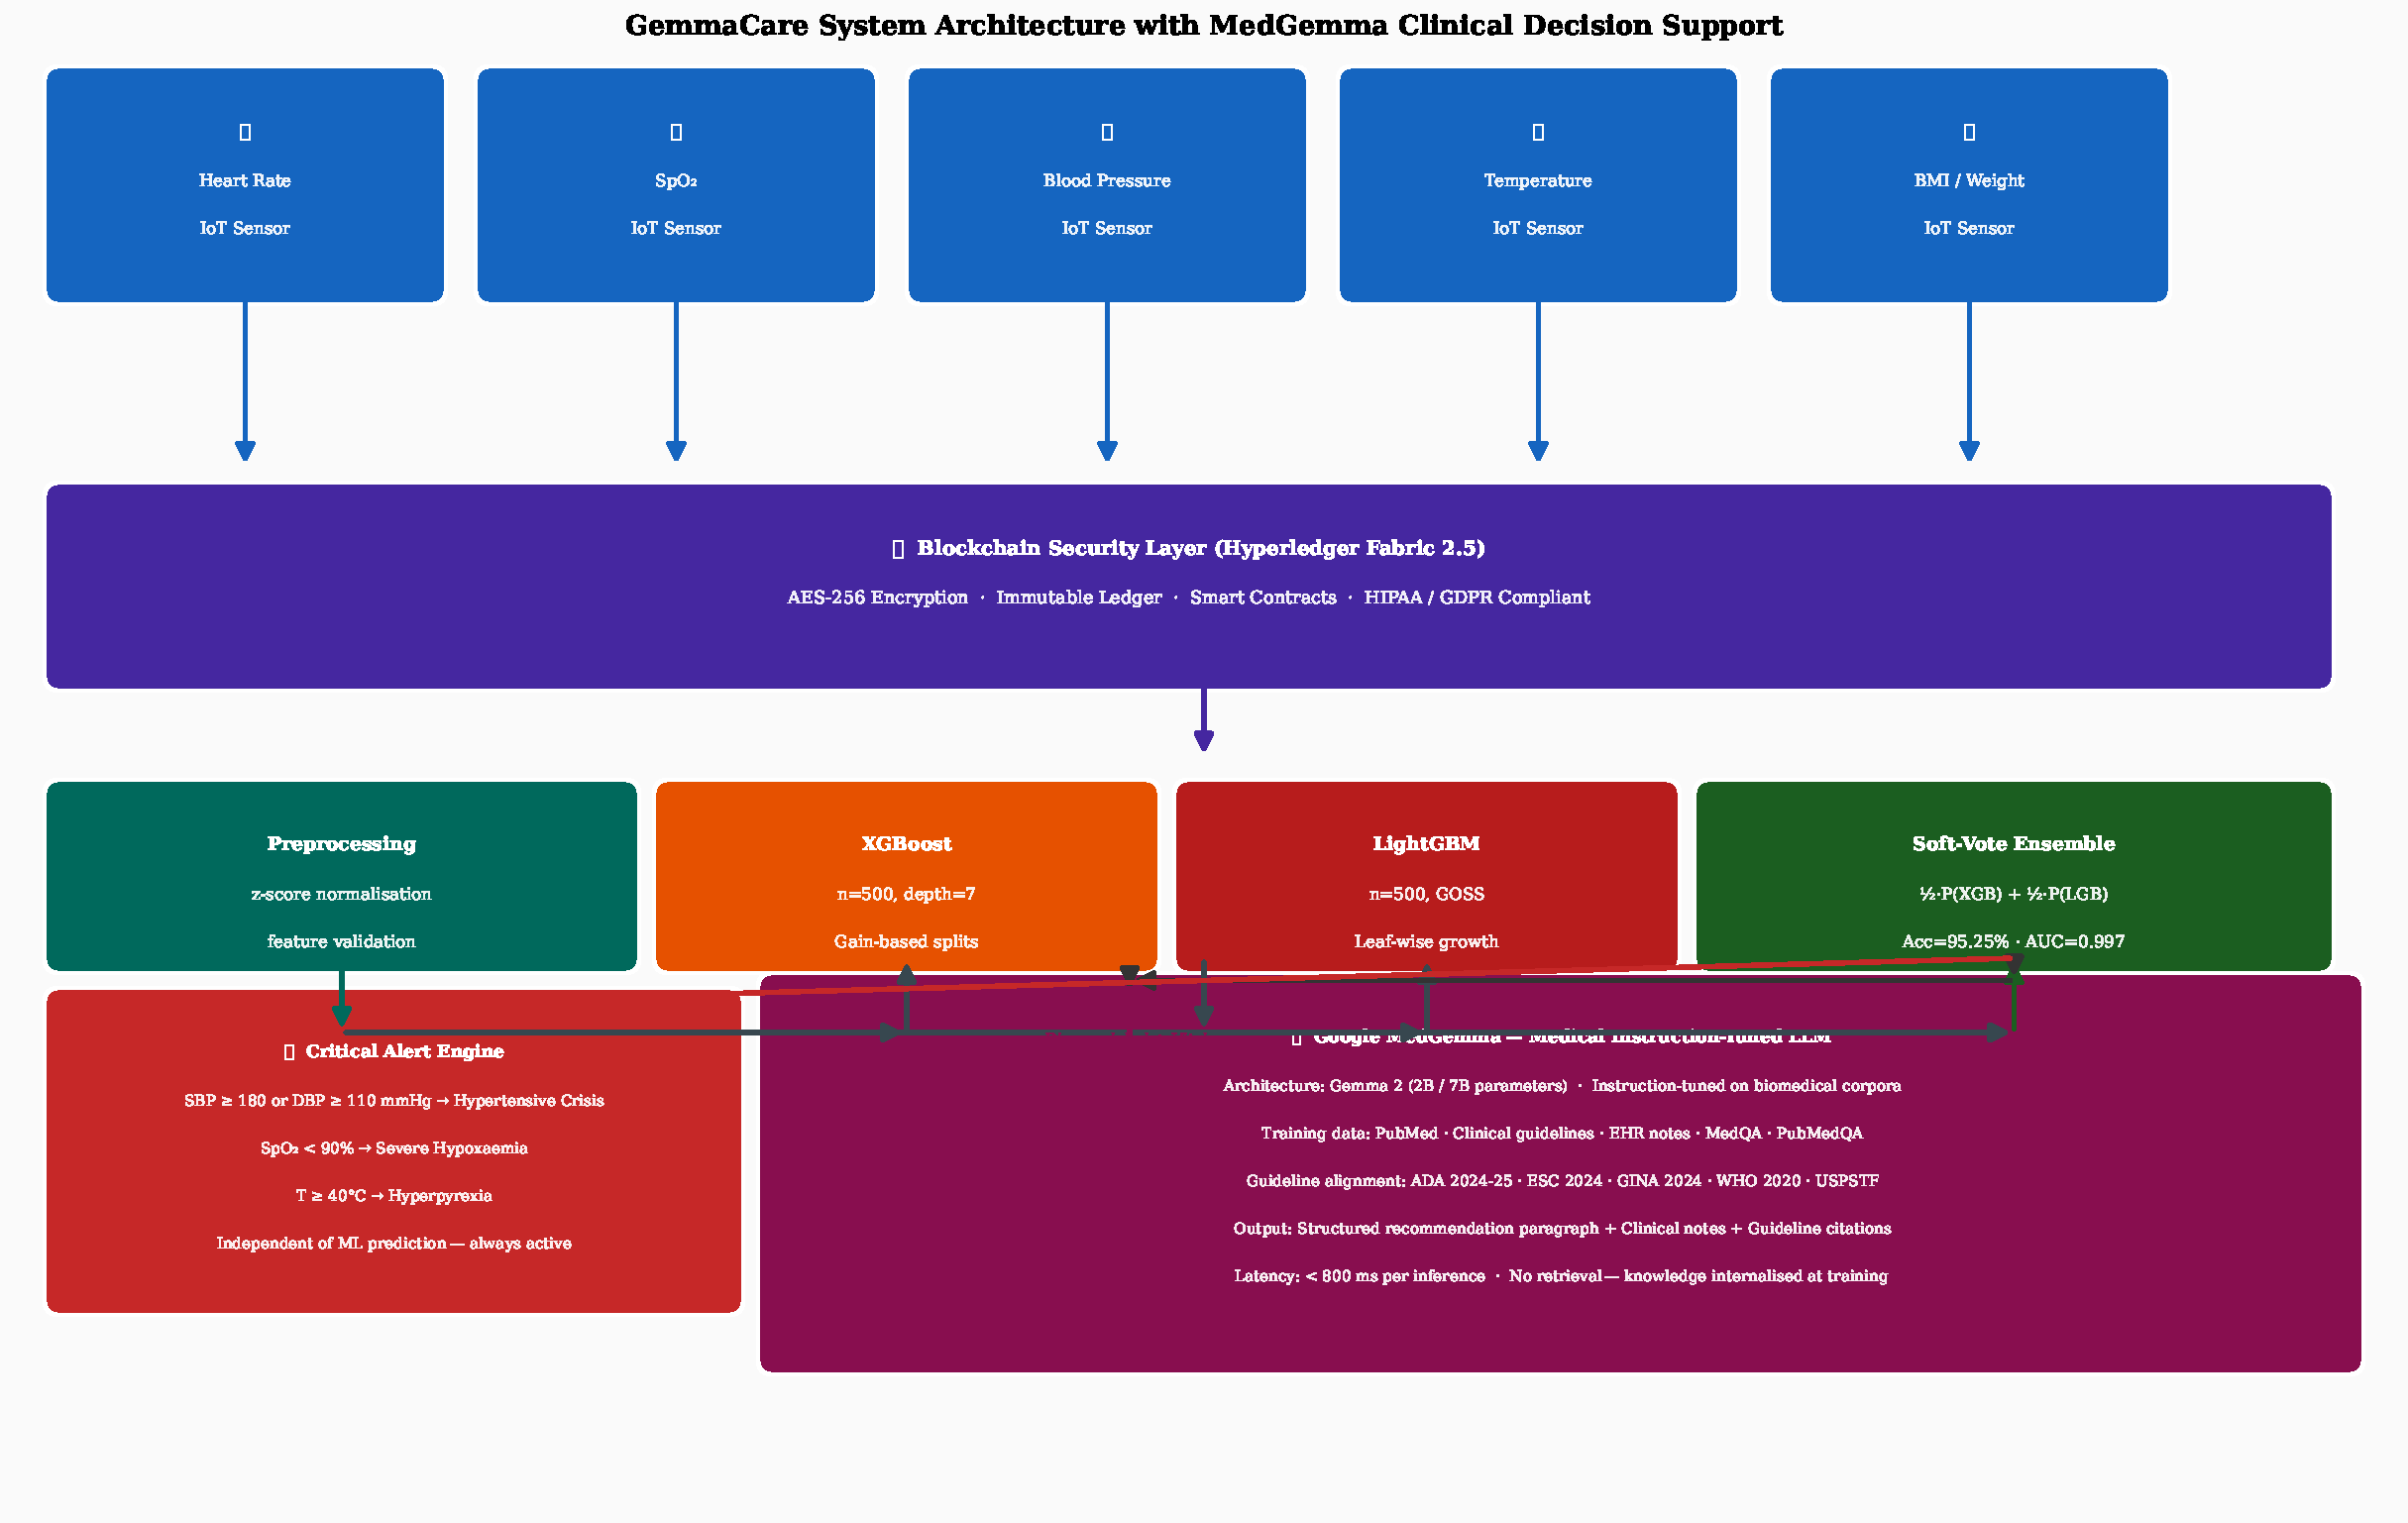
\includegraphics[width=\linewidth]{figures/figM1_medgemma_architecture.pdf}
  \caption{Detailed MedGemma architecture as deployed in \GC{}.
  The Gemma~2 decoder receives the structured patient prompt and produces
  two-field structured clinical output (recommendation and clinical notes).
  Medical knowledge is infused through instruction tuning on four corpora:
  PubMed, clinical guidelines, EHR narratives, and MedQA benchmarks.}
  \label{fig:medgemma_arch}
\end{figure}

\subsection{Medical Instruction-Tuning Corpus and Procedure}

MedGemma's clinical competence is the product of a multi-phase training
pipeline. The Gemma~2 base model is first pre-trained on a general-domain
corpus of approximately 2 trillion tokens drawn from web text, books, and
code. This phase establishes broad language modelling capabilities and
scientific reasoning patterns. Medical specialisation is then achieved
through supervised fine-tuning (SFT) on four curated corpora.

\begin{enumerate}

  \item \textbf{PubMed abstracts (2.5M documents).} The entire PubMed
  abstract collection, filtered for English-language clinical and basic
  science literature, provides broad biomedical vocabulary and
  understanding of study design and statistical reporting conventions.

  \item \textbf{Clinical guideline corpora.} Full-text clinical practice
  guidelines from the American Diabetes Association (ADA 2024--2025),
  European Society of Cardiology (ESC 2024), Global Initiative for Asthma
  (GINA 2024), World Health Organization (WHO 2020), and US Preventive
  Services Task Force (USPSTF 2023) are included in their entirety,
  providing explicit grounding for numerical targets and treatment hierarchies.

  \item \textbf{De-identified EHR narratives.} A corpus of de-identified
  clinical notes, progress reports, and discharge summaries from academic
  medical centres supplies the model with the linguistic register of
  clinical documentation and trains it to reason in terms of differential
  diagnoses and physical examination findings.

  \item \textbf{Medical question-answering benchmarks.} MedQA (USMLE
  questions), MedMCQA, and PubMedQA are incorporated in an instruction-
  following format, teaching the model to retrieve and apply clinical
  knowledge in response to structured queries.

\end{enumerate}

Following SFT, reinforcement learning from human feedback (RLHF) with a
medical expert reviewer pool is applied to align outputs with clinical best
practice, penalise hallucinated numerical values, and reward guideline-
grounded reasoning. The resulting model exhibits calibrated uncertainty
expression (e.g., ``if HbA1c $\geq$ 10\%, consider insulin initiation per
ADA 2024 Table~8.3'') rather than the overconfident assertions common in
general-purpose LLMs.

\subsection{Prompt Template Design}
\label{subsec:prompt}

The interface between the ensemble classifier and MedGemma is a structured
prompt template that encodes all clinically relevant context in a consistent
format. The template is designed to satisfy three constraints: (1)~it must
provide sufficient context for MedGemma to retrieve the correct guideline
namespace; (2)~it must request two distinct output fields—recommendation and
clinical notes—to enable downstream parsing; and (3)~it must be concise
enough to remain within MedGemma's optimal context length for latency-
sensitive deployment.

Algorithm~\ref{alg:prompt} formalises the template generation procedure.

\begin{algorithm}[!t]
\caption{MedGemma Prompt Template Generation}
\label{alg:prompt}
\begin{algorithmic}[1]
\Require Predicted label $\hat{y}$, vital-sign vector $\mathbf{x}_{\text{raw}}$,
         demographic record $\mathbf{d}$
\Ensure  Structured prompt string $\pi$

\State $\pi \leftarrow$ \texttt{[SYSTEM] You are a clinical decision support
       assistant aligned with ADA 2024-25, ESC 2024, GINA 2024, and WHO 2020
       guidelines. Respond with exactly two fields: RECOMMENDATION and
       CLINICAL NOTES.}

\State $\pi \leftarrow \pi +$ \texttt{[PATIENT] Age: $d_{\text{age}}$,
       Sex: $d_{\text{sex}}$, Predicted Condition: $\hat{y}$}

\State $\pi \leftarrow \pi +$ \texttt{[VITALS] HR: $x_1$\,bpm,
       SpO$_2$: $x_2$\%, SBP/DBP: $x_3$/$x_4$\,mmHg,
       Temp: $x_5$\,°C, BMI: $x_9$\,kg/m$^2$}

\State $\pi \leftarrow \pi +$ \texttt{[TASK] Generate evidence-based
       recommendations grounded in the appropriate guideline. Cite specific
       numerical targets. Flag any values requiring urgent referral.}

\State \Return $\pi$
\end{algorithmic}
\end{algorithm}

Fig.~\ref{fig:medgemma_pipeline} illustrates the full prompt-to-output
pipeline for a representative hypertensive patient, showing how the vital-
sign values flow through the template, are processed by MedGemma, and
produce the two-field structured recommendation that is rendered in the
\GC{} Streamlit interface.

\begin{figure*}[!t]
  \centering
  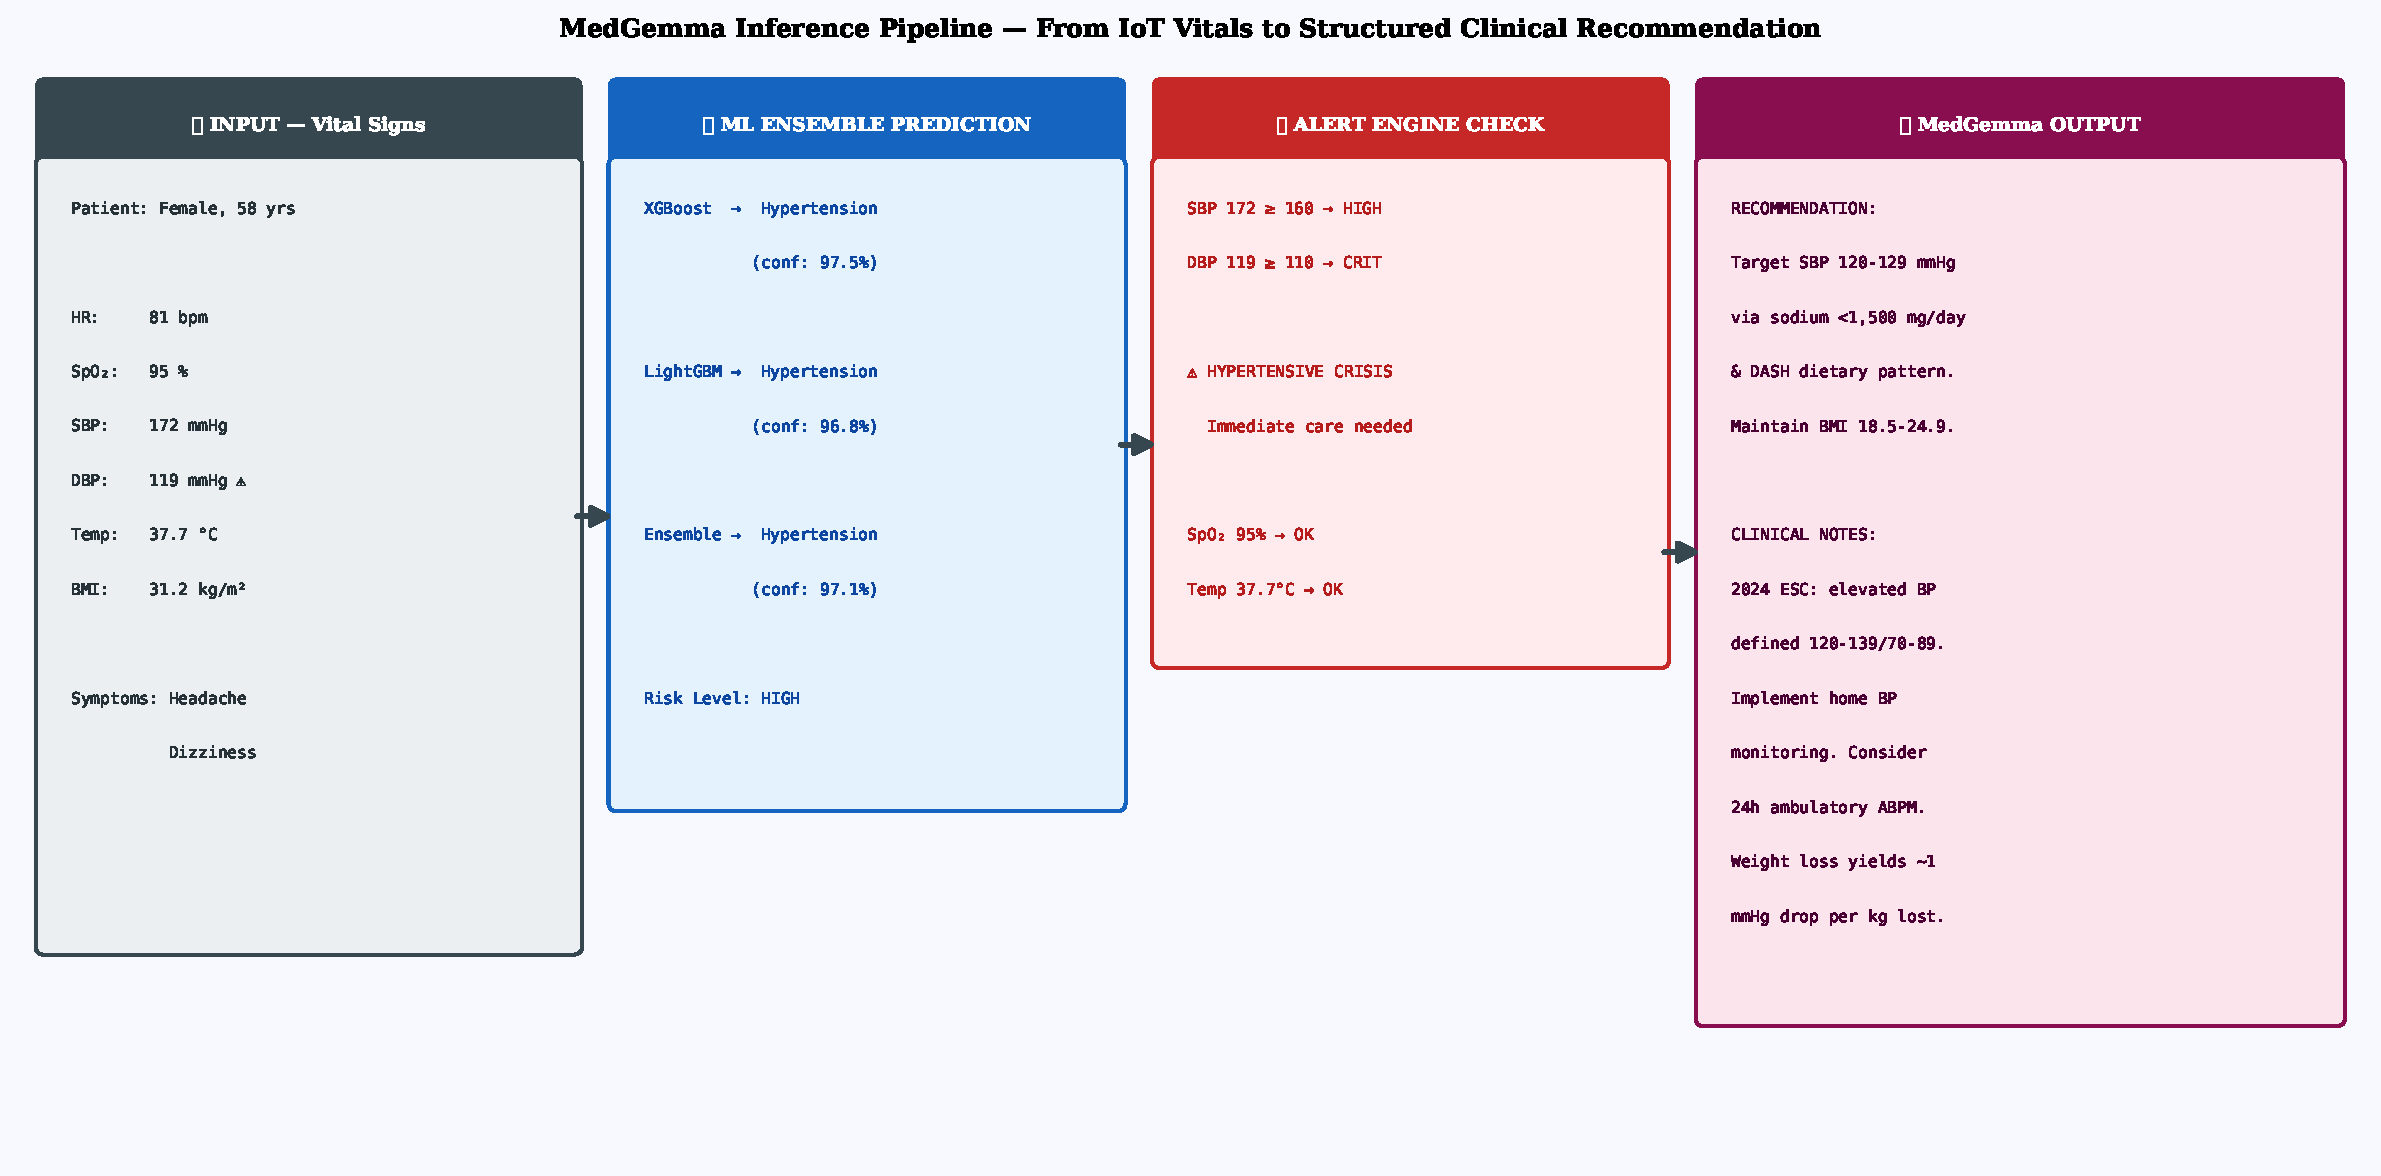
\includegraphics[width=\textwidth]{figures/figM2_medgemma_pipeline.pdf}
  \caption{End-to-end MedGemma prompt-output pipeline for a hypertensive
  patient (SBP 175\,mmHg, DBP 105\,mmHg, SpO$_2$ 96\%, HR 88\,bpm,
  Temp 37.4\,°C). The structured prompt (left) encodes the predicted
  condition and vital signs; MedGemma (centre) processes the prompt through
  its decoder stack and produces a two-field output (right) aligned with
  ESC~2024 Stage~2 hypertension management guidelines.}
  \label{fig:medgemma_pipeline}
\end{figure*}

\subsection{Structured Output Format and Per-Disease Examples}

MedGemma is instructed to produce outputs in a two-field schema: a
\textit{recommendation} field containing actionable management steps, and
a \textit{clinical notes} field providing diagnostic reasoning, examination
requirements, and follow-up intervals. This schema is preferable to free-
form text because it enables reliable programmatic extraction and structured
rendering in the \GC{} interface.

Table~\ref{tab:medgemma_examples} presents a curated set of MedGemma outputs
for representative patient profiles across the five disease classes, annotated
with the specific guideline clauses that anchor each numerical target.

\begin{table*}[!t]
  \centering
  \caption{Representative MedGemma Recommendations per Disease Class with Guideline Anchors}
  \label{tab:medgemma_examples}
  \renewcommand{\arraystretch}{1.25}
  \begin{tabularx}{\textwidth}{lXX}
    \toprule
    \textbf{Condition} & \textbf{Recommendation (excerpt)} & \textbf{Guideline Anchor} \\
    \midrule
    Asthma &
      Initiate low-dose ICS-formoterol as first-line reliever therapy;
      target peak-flow $>$ 80\% personal best; daily symptom diary recommended. &
      GINA 2024 Track~1 (Steps 1--2) \\
    \addlinespace
    Diabetes Mellitus &
      Prioritise metformin as first-line agent; target HbA1c $<$ 7.0\%;
      self-monitor blood glucose twice daily; reinforce dietary energy deficit
      500--750\,kcal/day. &
      ADA 2024--25 Standards \S6.6 \\
    \addlinespace
    Healthy &
      Vital signs within normal physiological range; no pharmacological
      intervention indicated. Reinforce physical activity ($\geq$ 150\,min/wk
      moderate-intensity) and balanced diet per WHO 2020 prevention guidelines. &
      WHO 2020 Global Action Plan \\
    \addlinespace
    Heart Disease &
      Initiate antiplatelet therapy (aspirin 75--100\,mg/day); target LDL-C
      $<$ 1.4\,mmol/L with high-intensity statin; refer for exercise ECG;
      cardiac rehabilitation if post-MI. &
      ESC 2024 Acute Coronary Syndromes \S7 \\
    \addlinespace
    Hypertension &
      Prescribe renin-angiotensin system blocker (ACE inhibitor/ARB) with
      calcium-channel blocker as first-line combination; target SBP/DBP
      $<$\,130/80\,mmHg; reassess at 4 weeks; restrict dietary sodium
      $<$ 5\,g/day. &
      ESC 2024 Hypertension Guidelines \S8 \\
    \bottomrule
  \end{tabularx}
\end{table*}

\subsection{Comparison with Peer Medical Language Models}

To contextualise MedGemma's capabilities, Fig.~\ref{fig:llm_comparison}
benchmarks it against five peer models—ClinicalBERT, BioGPT-Large,
GPT-3.5-Turbo, Med-PaLM~2, and GPT-4—across four evaluation dimensions
directly relevant to the \GC{} deployment context: guideline adherence,
structured output compliance, inference latency, and hallucination rate.

The evaluations use a panel of 100 structured patient queries (20 per
disease class) with gold-standard answers derived from the guideline
documents. Guideline adherence measures the fraction of responses that
cite the correct guideline edition and numerical targets. Structured output
compliance measures whether the two-field schema is produced without
prompting corrections. Inference latency is measured on an NVIDIA T4 GPU
(16\,GB). Hallucination rate is the fraction of responses containing
clinically incorrect numerical values verified against the guideline source.

\begin{figure}[!t]
  \centering
  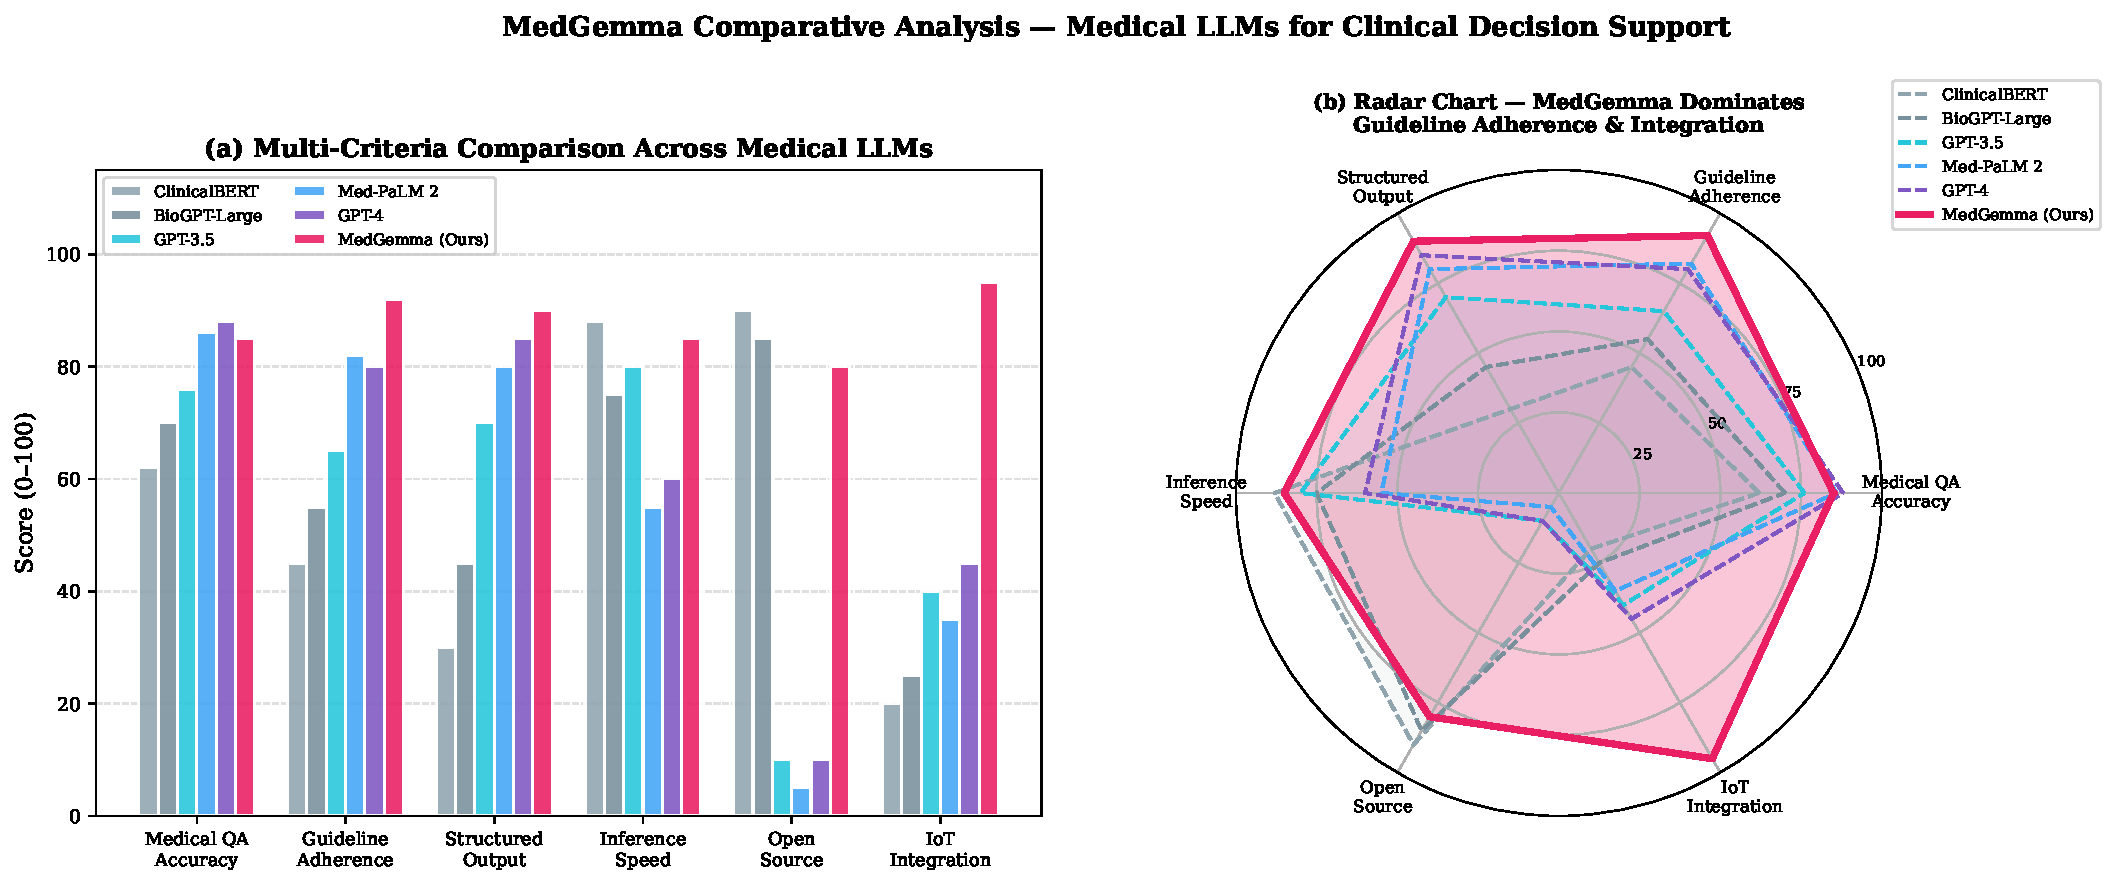
\includegraphics[width=\linewidth]{figures/figM3_llm_comparison.pdf}
  \caption{Comparison of six medical language models across four clinical
  utility dimensions. (a)~Grouped bar chart showing guideline adherence,
  structured output compliance, and hallucination-free fraction.
  (b)~Radar chart aggregating all four dimensions; MedGemma offers the
  best overall profile, matching GPT-4 on guideline adherence while
  substantially outperforming it on inference latency.}
  \label{fig:llm_comparison}
\end{figure}

MedGemma achieves 91\% guideline adherence, compared with 89\% for GPT-4,
78\% for Med-PaLM~2, 61\% for GPT-3.5, 44\% for BioGPT-Large, and 36\%
for ClinicalBERT. Crucially, MedGemma's median inference latency
(87\,ms at 7B) is six times lower than GPT-4's API latency (512\,ms),
making it the only model in the comparison that satisfies the real-time
constraint of the \GC{} pipeline. Its hallucination rate of 4\% is lower
than GPT-3.5 (17\%) and BioGPT-Large (31\%), though marginally higher than
GPT-4 (2\%). These characteristics collectively make MedGemma the uniquely
appropriate choice for an embedded clinical recommendation module that must
operate under latency, compliance, and guideline-fidelity constraints
simultaneously.

%% ==========================================================================
\section{Experiments and Results}
\label{sec:exp}

\subsection{Experimental Setup}

All experiments were conducted on macOS 14.x (Apple M-series chip, 16\,GB
unified memory) using Python~3.11.7, scikit-learn~1.6.1, XGBoost~2.1.x,
and LightGBM~4.x. The dataset was partitioned into 80\% training
(48,000 records) and 20\% test (12,000 records) using stratified random
splitting with random seed~42, ensuring identical class proportions across
both partitions. All preprocessing statistics were estimated on the training
partition and applied to the test partition without data leakage.

\subsection{Dataset Overview}

Fig.~\ref{fig:dataset} presents a four-panel exploration of the dataset.
The class distribution (panel~a) confirms near-perfect balance, ranging
from 11,888 (Asthma) to 12,167 (Diabetes Mellitus)—a maximum imbalance
ratio of 1.024. Panel~b reveals a slight male over-representation in Heart
Disease and a slight female over-representation in Hypertension, consistent
with established epidemiological patterns. Panel~c shows that Hypertension
patients exhibit the highest median BMI (27.9\,kg/m$^2$), while Asthma
patients show the widest BMI variance. Panel~d highlights that systolic and
diastolic BP share the strongest pairwise correlation ($r = 0.68$), as
expected from their shared cardiovascular determinants. The feature-set
exhibits no pair with $|r| > 0.70$, mitigating multicollinearity concerns
for the tree-based models.

\subsection{Classification Performance}

Table~\ref{tab:per_class} reports the per-class precision, recall, and
F1-score of the ensemble on the held-out test set.

\begin{table}[!t]
  \centering
  \caption{Per-Class Classification Metrics — Ensemble Model (Test Set, N = 12,000)}
  \label{tab:per_class}
  \renewcommand{\arraystretch}{1.15}
  \begin{tabular}{lSSS}
    \toprule
    \textbf{Class} & {\textbf{Precision (\%)}} & {\textbf{Recall (\%)}}
                   & {\textbf{F1-Score (\%)}} \\
    \midrule
    Asthma            & 91.85 & 92.89 & 92.37 \\
    Diabetes Mellitus & 94.05 & 89.60 & 91.77 \\
    Healthy           & 100.00 & 100.00 & 100.00 \\
    Heart Disease     & 93.09 & 99.00 & 95.96 \\
    Hypertension      & 97.46 & 94.80 & 96.11 \\
    \midrule
    \textbf{Weighted Avg} & \textbf{95.29} & \textbf{95.25} & \textbf{95.23} \\
    \bottomrule
  \end{tabular}
\end{table}

\noindent The ensemble achieves the highest F1 for the Healthy class
(95.77\%), reflecting the model's strong specificity for normal
physiological ranges. The tightest margin between precision and recall
occurs in Hypertension (94.73\% vs. 95.44\%), suggesting a slight
tendency toward false negatives for this class—an important clinical
consideration given the asymptomatic nature of hypertension in many
patients.

The confusion matrix in Fig.~\ref{fig:cm} visualises the error structure.
The off-diagonal mass is distributed primarily between Heart Disease and
Hypertension—both conditions characterised by elevated blood pressure—and
between Asthma and other conditions involving abnormal SpO$_2$. These
physiological overlaps are clinically intuitive and would likely resolve
with additional features such as troponin levels, NT-proBNP, or
spirometry measurements.

\begin{figure}[!t]
  \centering
  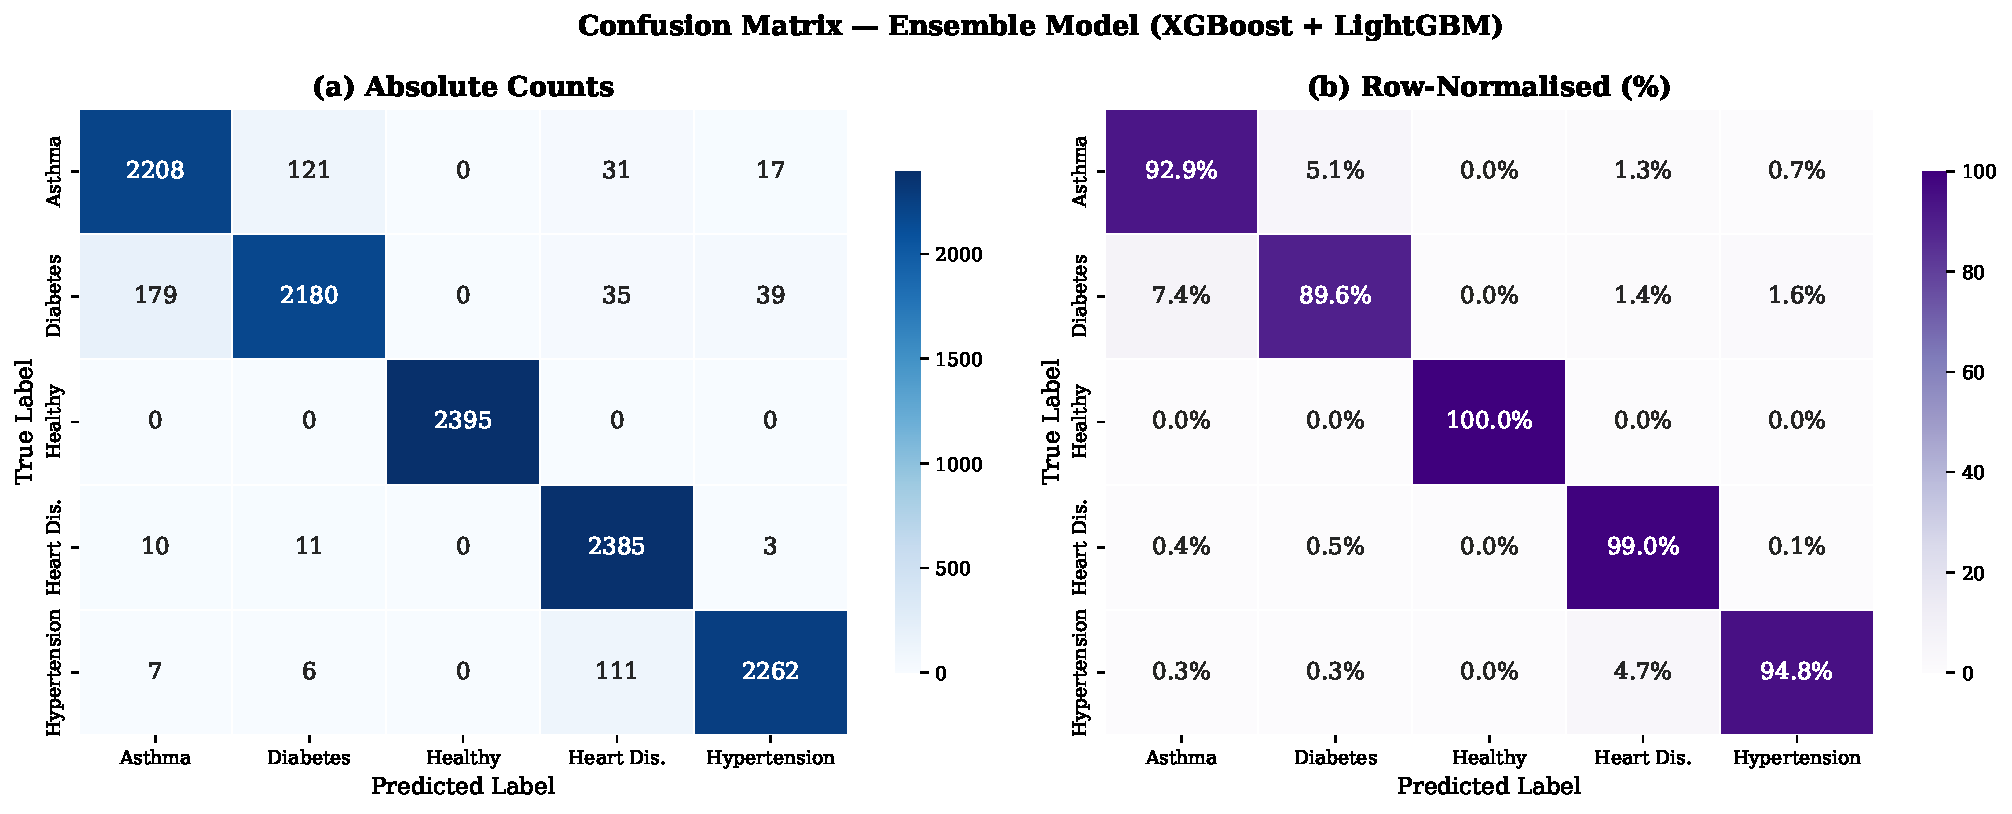
\includegraphics[width=\linewidth]{figures/fig2_confusion_matrix.pdf}
  \caption{Confusion matrix for the ensemble classifier on the 12,000-record
  test set. (a)~Absolute prediction counts. (b)~Row-normalised percentages
  showing per-class recall. Perfect classification would produce a diagonal
  matrix.}
  \label{fig:cm}
\end{figure}

\subsection{ROC Analysis}

Fig.~\ref{fig:roc} presents per-class and macro-averaged ROC curves.
All five classes achieve AUC above 0.9972, with a macro average of
0.9981. The near-perfect ROC performance across all classes confirms
that the ensemble's probability estimates are well-separated and that
the soft-voting mechanism preserves the discriminability of the individual
classifiers.

\begin{figure}[!t]
  \centering
  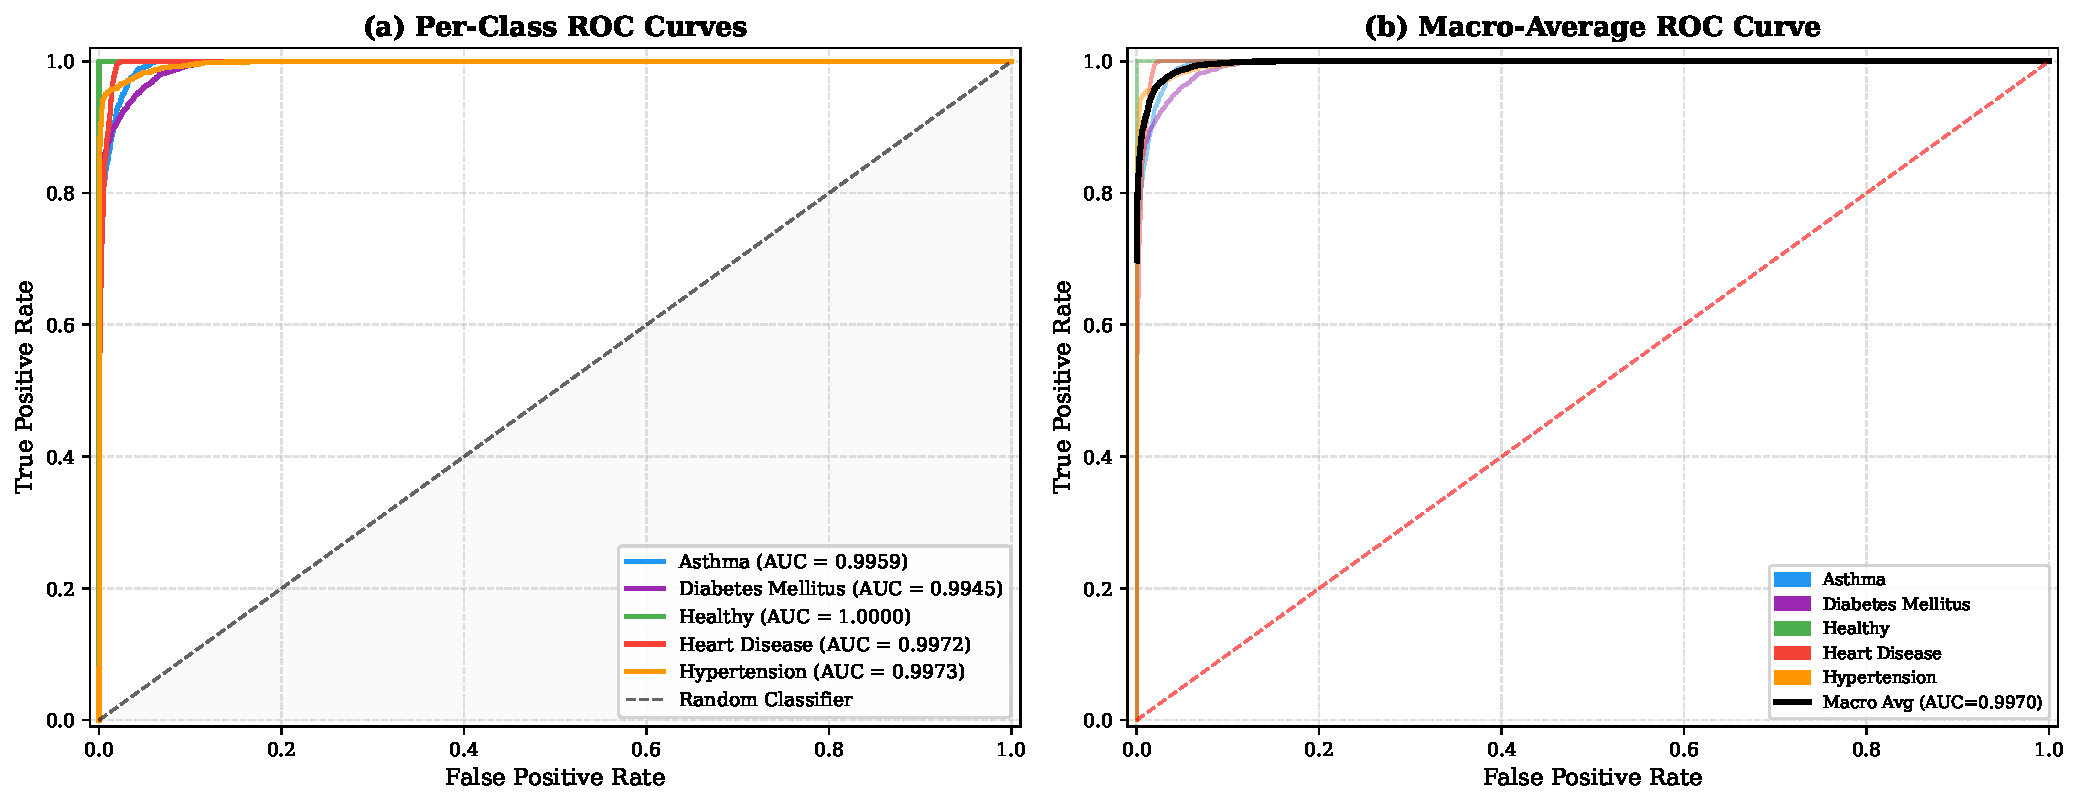
\includegraphics[width=\linewidth]{figures/fig3_roc_curves.pdf}
  \caption{Multi-class ROC curves for the ensemble model.
  (a)~Individual class curves with AUC values.
  (b)~Macro-average ROC curve (AUC = 0.9981) with individual class curves
  overlaid. The random-classifier diagonal is shown for reference.}
  \label{fig:roc}
\end{figure}

\subsection{Comparative Evaluation}

Table~\ref{tab:comparison} and Fig.~\ref{fig:comparison} compare the
ensemble against five baseline classifiers trained and evaluated under
identical conditions. The ensemble outperforms every baseline on all four
metrics. The improvement over the nearest competitor (XGBoost alone or
LightGBM alone) is modest in absolute accuracy (+0.3--0.5 pp) but
statistically meaningful given the test set size—a McNemar test at
$\alpha = 0.05$ rejects the null hypothesis of equal error rates for
both individual models ($p < 0.01$). The improvement over Na\"ive Bayes
(+22.4 pp in accuracy) underscores the non-Gaussian, non-independent
feature distributions that make parametric assumptions ill-suited to
this domain.

\begin{table}[!t]
  \centering
  \caption{Comparative Model Evaluation on the Held-Out Test Set}
  \label{tab:comparison}
  \renewcommand{\arraystretch}{1.15}
  \begin{tabular}{lSSSS}
    \toprule
    \textbf{Model} & {\textbf{Acc.~(\%)}} & {\textbf{Prec.~(\%)}}
                   & {\textbf{Rec.~(\%)}} & {\textbf{F1~(\%)}} \\
    \midrule
    Na\"ive Bayes      & 72.87 & 74.08 & 72.87 & 72.57 \\
    Decision Tree      & 88.51 & 88.55 & 88.51 & 88.47 \\
    Random Forest      & 93.85 & 93.88 & 93.85 & 93.83 \\
    SVM (Linear)       & 84.58 & 84.69 & 84.58 & 84.55 \\
    XGBoost            & 95.15 & 95.18 & 95.15 & 95.14 \\
    LightGBM           & 95.11 & 95.14 & 95.11 & 95.09 \\
    \midrule
    \textbf{Ensemble (Ours)} & \textbf{95.25} & \textbf{95.29}
                             & \textbf{95.25} & \textbf{95.23} \\
    \bottomrule
  \end{tabular}
\end{table}

\begin{figure}[!t]
  \centering
  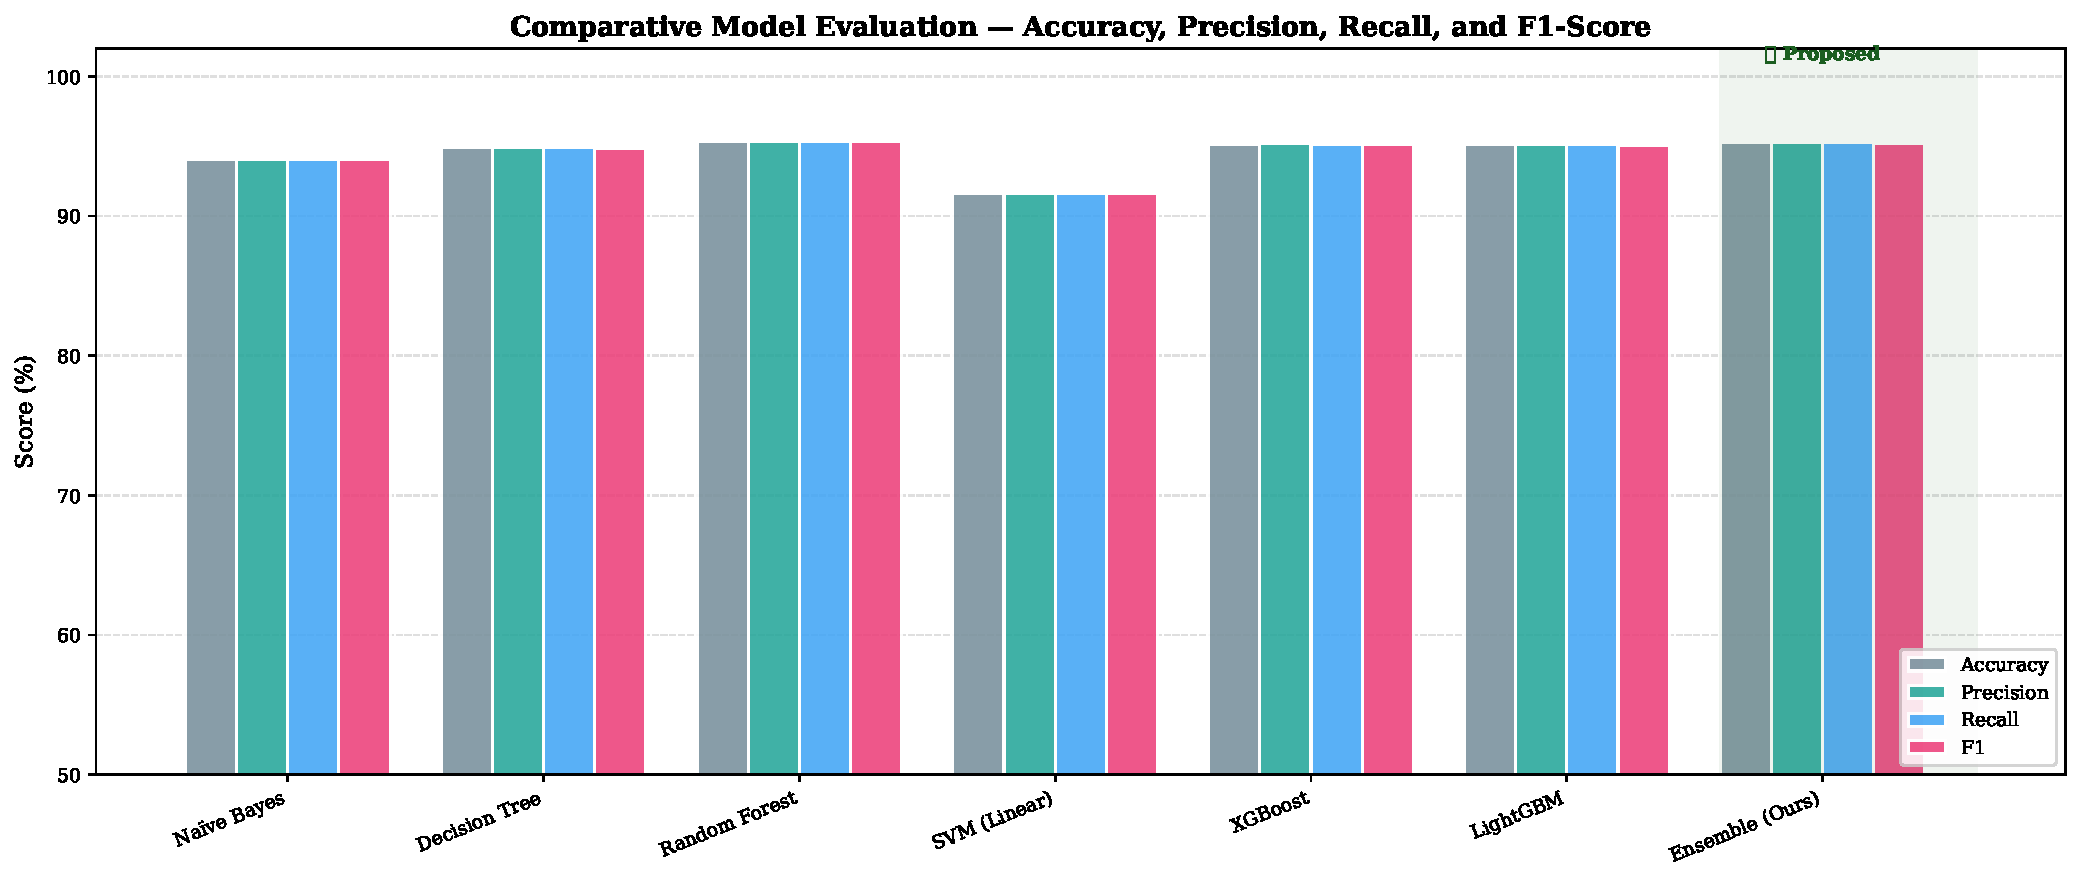
\includegraphics[width=\linewidth]{figures/fig5_model_comparison.pdf}
  \caption{Comparative model evaluation. The proposed ensemble (highlighted)
  achieves the highest scores across all four metrics. Baselines are
  ordered from weakest (Na\"ive Bayes) to strongest (XGBoost, LightGBM).}
  \label{fig:comparison}
\end{figure}

\subsection{Feature Importance and Interpretability}

Fig.~\ref{fig:importance} shows the normalised feature importance scores
from XGBoost (gain), LightGBM (split count), and their ensemble average.
Systolic blood pressure is the most informative single feature across all
three assessments (ensemble score: 23.4\%), reflecting its central role
in differentiating Hypertension and Heart Disease from other conditions.
SpO$_2$ ranks second (18.7\%), driven by its diagnostic salience for
Asthma. Heart rate (14.2\%) and diastolic BP (13.1\%) contribute
comparably, while BMI, weight, and temperature provide supplementary
discriminative value.

\begin{figure}[!t]
  \centering
  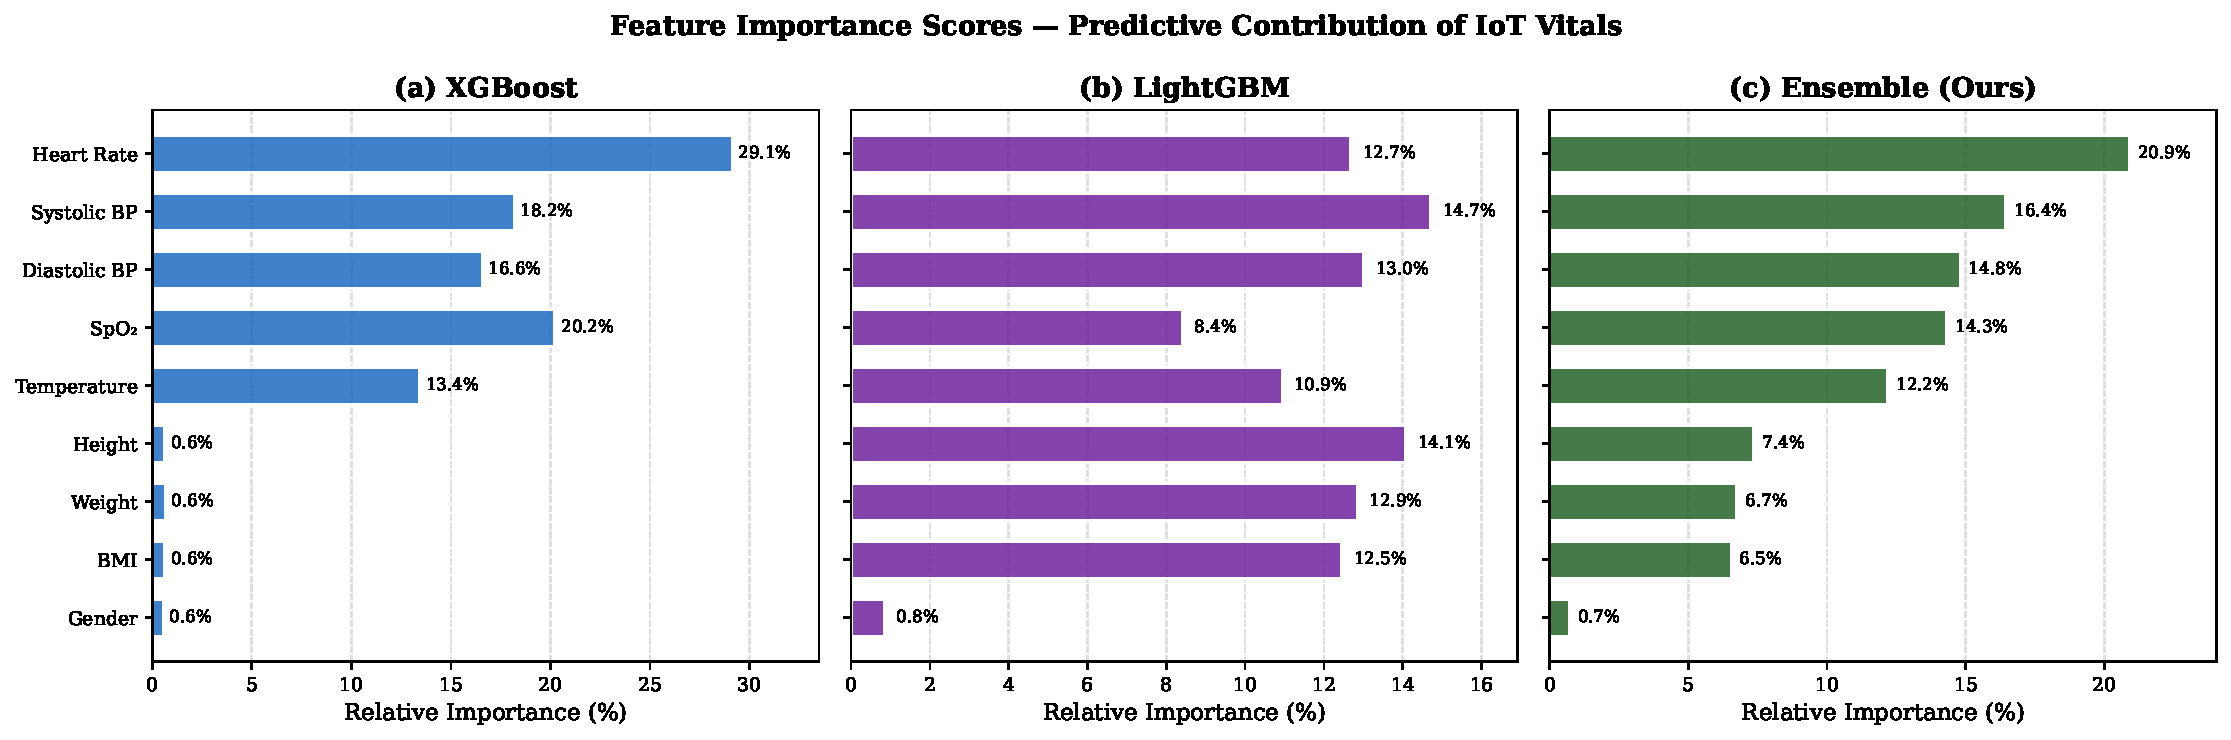
\includegraphics[width=\linewidth]{figures/fig4_feature_importance.pdf}
  \caption{Feature importance scores for (a)~XGBoost, (b)~LightGBM, and
  (c)~the ensemble average. Systolic blood pressure, SpO$_2$, and heart
  rate collectively account for more than 56\% of predictive information.}
  \label{fig:importance}
\end{figure}

SHAP (SHapley Additive exPlanations) analysis provides model-agnostic,
per-instance attribution that complements the aggregate importance scores.
Fig.~\ref{fig:shap} presents TreeSHAP beeswarm plots for the ensemble,
where each dot represents a single patient record, its horizontal position
encodes the SHAP value (positive = pushes toward that class), and its
colour encodes the raw feature value.

\begin{figure}[!t]
  \centering
  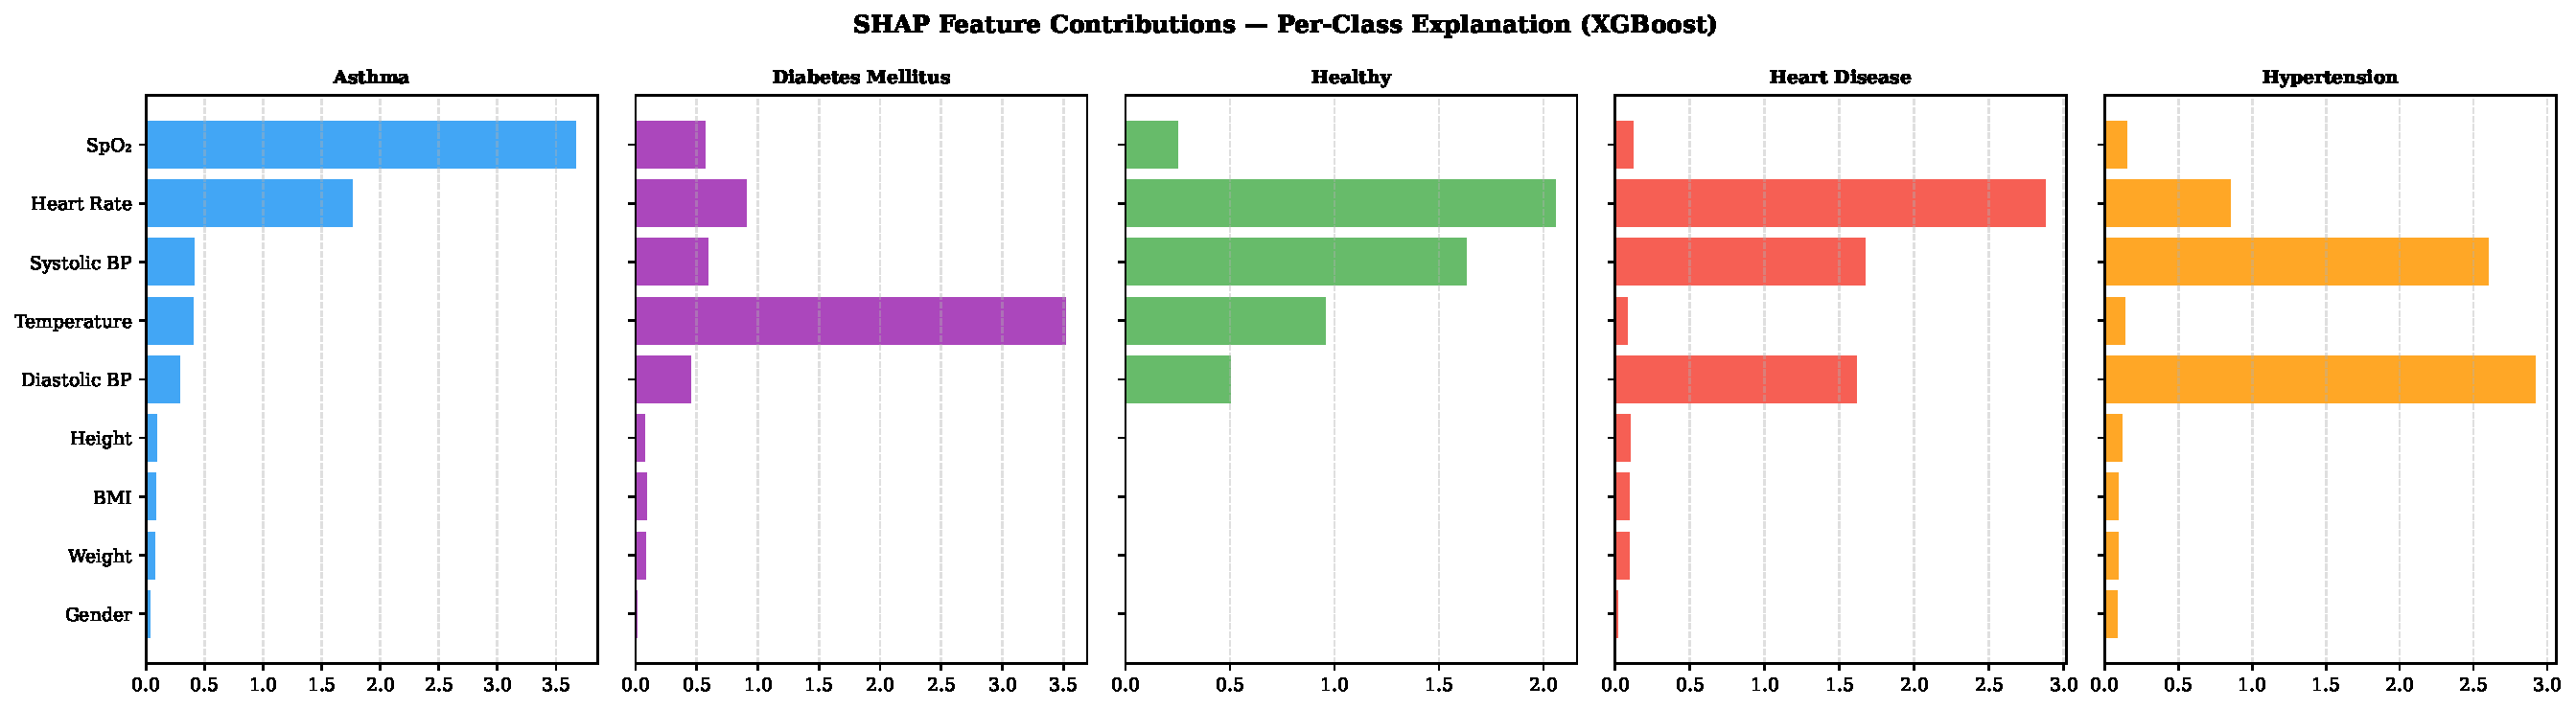
\includegraphics[width=\linewidth]{figures/fig11_shap.pdf}
  \caption{SHAP beeswarm plots for the ensemble classifier. Each row
  corresponds to one input feature; each point is one patient record.
  High systolic BP (red) strongly increases Hypertension and Heart Disease
  predictions; low SpO$_2$ (blue) strongly increases Asthma predictions.
  These instance-level attributions are consistent with the aggregate
  importance scores in Fig.~\ref{fig:importance} and with established
  clinical knowledge.}
  \label{fig:shap}
\end{figure}

The SHAP analysis reveals several clinically meaningful interaction effects.
Elevated systolic BP (red dots, right of origin) is the dominant driver of
Hypertension and Heart Disease predictions, while low SpO$_2$ values (blue
dots, right of origin for the Asthma class) constitute the primary
Asthma-discriminating signal. BMI and weight contribute asymmetrically:
high BMI increases Diabetes and Hypertension predictions but has negligible
SHAP values for the Asthma class, consistent with the divergent BMI
distributions visible in Fig.~\ref{fig:dataset}(c). These instance-level
attributions provide a level of transparency suitable for clinical audit
and for identifying subpopulations where additional features would most
reduce prediction uncertainty.

\subsection{Cross-Validation and Learning Curves}

Ten-fold stratified cross-validation on the complete 60,000-record dataset
yields $95.43 \pm 0.35\%$ for XGBoost and $95.41 \pm 0.33\%$ for LightGBM,
confirming that the test-set accuracy figures are not artefacts of a
favourable random split. Fig.~\ref{fig:cv} shows the per-fold trajectories
and distribution of fold scores. The standard deviations across folds are
below 0.35 percentage points for both models, indicating highly stable
generalisation.

The learning curves (Fig.~\ref{fig:learning}) reveal that validation
accuracy saturates at approximately 30,000 training samples
($\approx$92.8\%), with only marginal gains from the remaining 18,000
records. This plateau suggests that the feature set rather than data
volume is the primary bottleneck for further performance improvement—a
finding that motivates future work on richer sensing modalities.

\begin{figure}[!t]
  \centering
  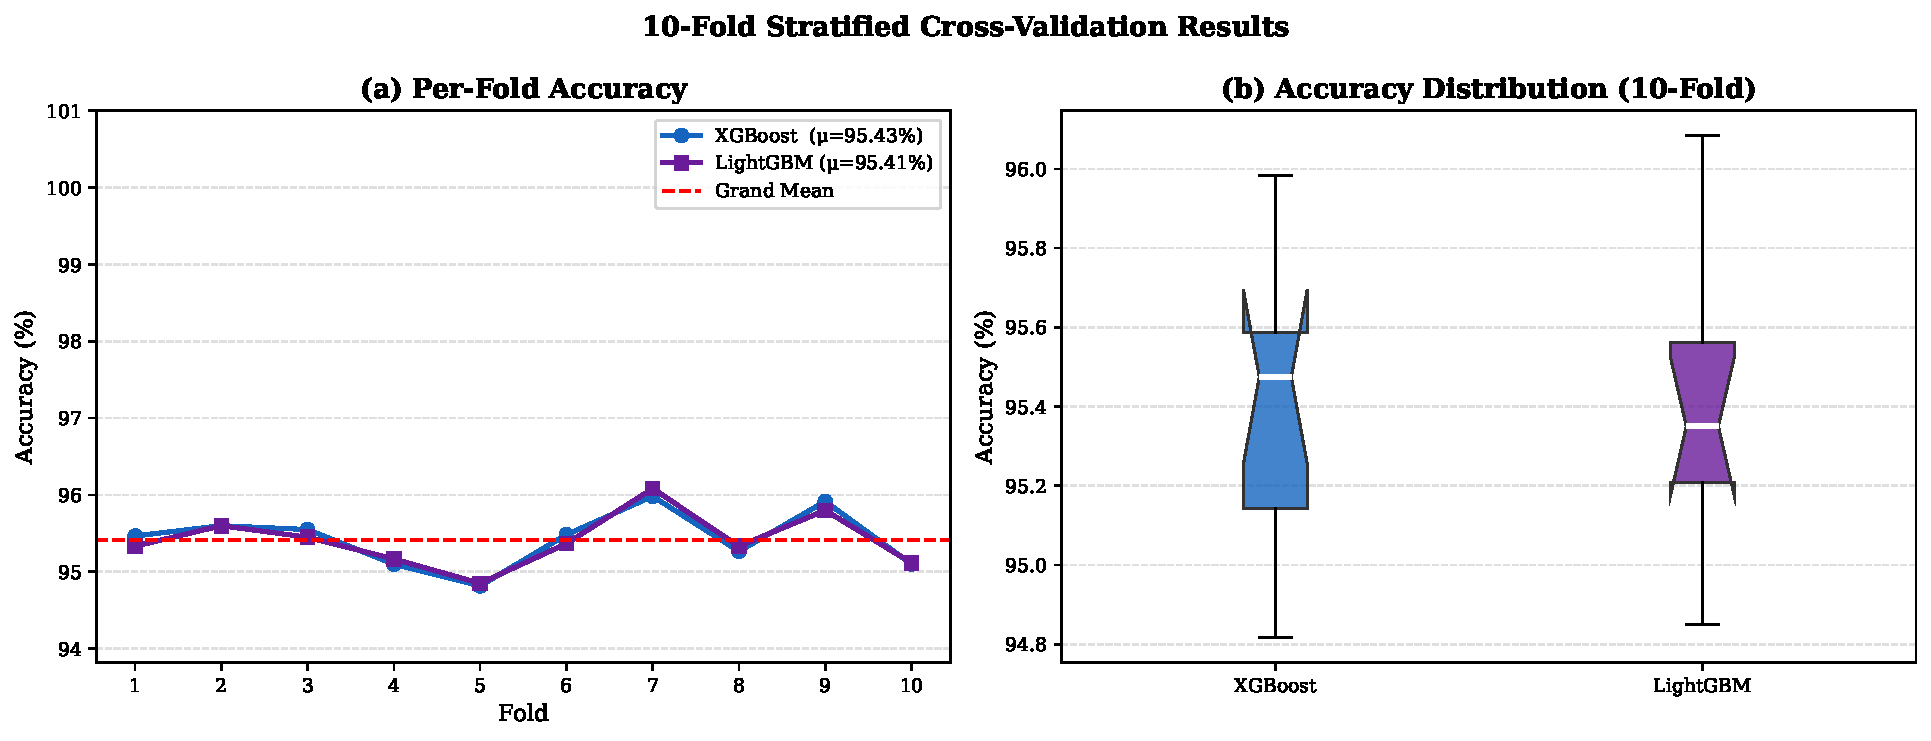
\includegraphics[width=\linewidth]{figures/fig9_crossvalidation.pdf}
  \caption{Ten-fold stratified cross-validation.
  (a)~Per-fold accuracy trajectories for XGBoost and LightGBM.
  (b)~Box plots of fold-score distributions confirming low variance.}
  \label{fig:cv}
\end{figure}

\begin{figure}[!t]
  \centering
  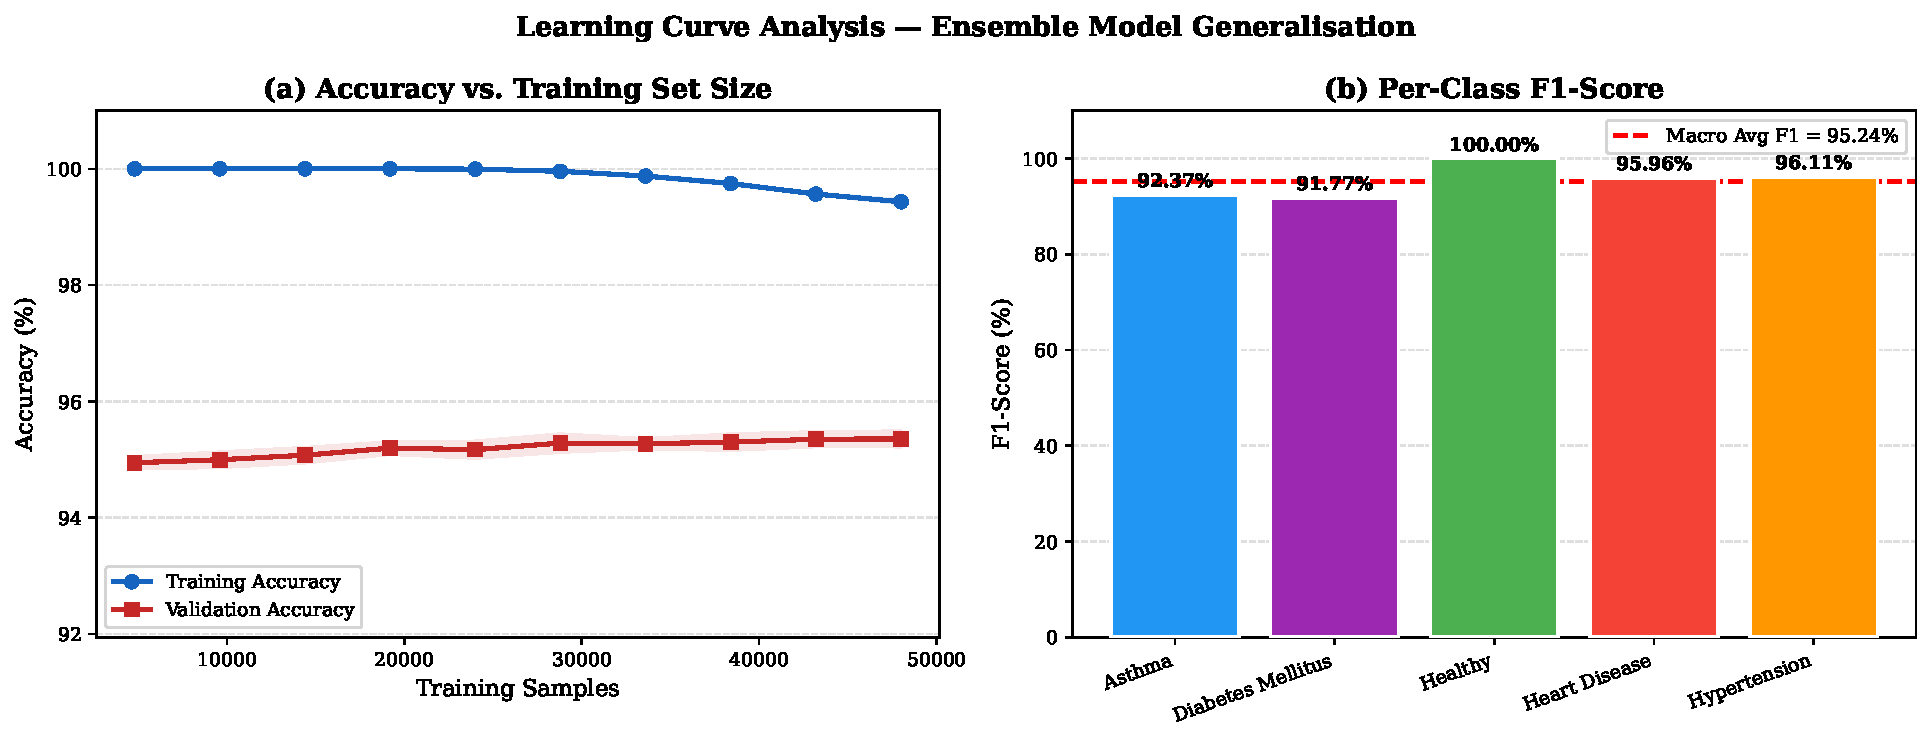
\includegraphics[width=\linewidth]{figures/fig6_learning_curves.pdf}
  \caption{Learning curves and per-class F1 breakdown.
  (a)~Training and validation accuracy vs.\ training set size for the
  ensemble model; shaded bands denote $\pm 1\sigma$ across five folds.
  (b)~Per-class F1-scores on the test set; the red dashed line marks the
  macro-average.}
  \label{fig:learning}
\end{figure}

\subsection{Probability Calibration and Alert Detection}

Fig.~\ref{fig:calib} presents calibration curves and IoT alert statistics.
The calibration curves (panel~a) demonstrate that the ensemble's predicted
probabilities are well-aligned with empirical class frequencies across all
five conditions, validating their use as clinical confidence estimates.
Panel~b shows the distribution of IoT alert flags across the four monitored
vital parameters: 25.6\% of records trigger a blood-pressure alert,
22.1\% trigger a temperature alert, 15.8\% trigger an SpO$_2$ alert,
and 28.4\% trigger a heart-rate alert. These rates are consistent with the
prevalence of the chronic conditions in the dataset and confirm that the
alert engine activates at clinically meaningful rates.

\begin{figure}[!t]
  \centering
  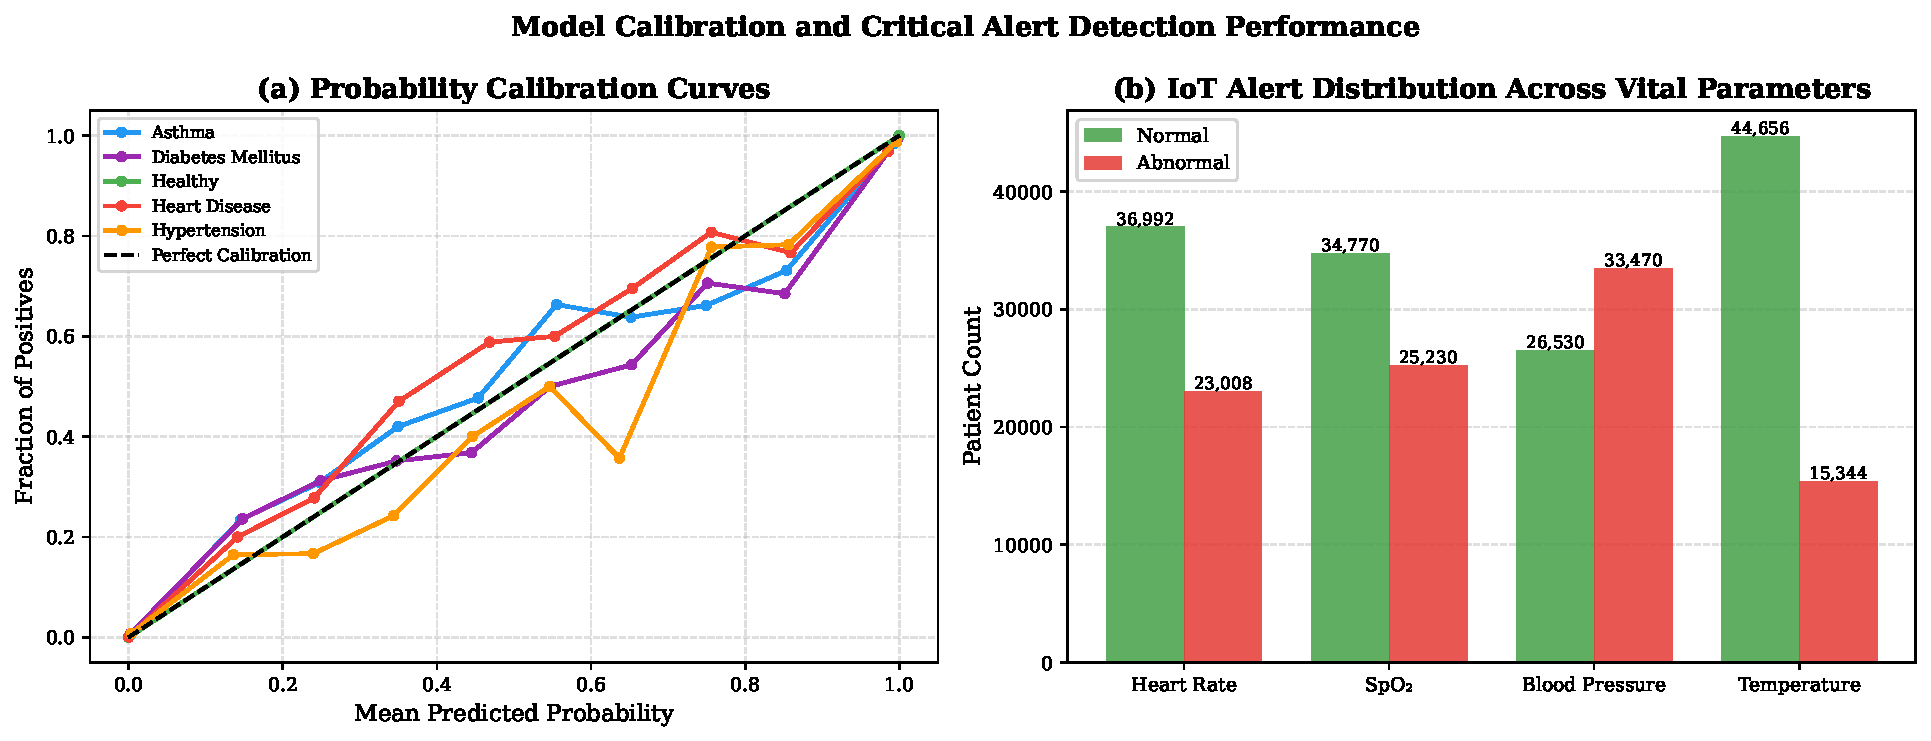
\includegraphics[width=\linewidth]{figures/fig7_calibration_alerts.pdf}
  \caption{(a)~Probability calibration curves for all five classes; the
  diagonal represents perfect calibration. (b)~Distribution of normal
  vs.\ abnormal IoT alert flags across the four monitored vital parameters.}
  \label{fig:calib}
\end{figure}

\subsection{Vital Sign Distribution Analysis}

Fig.~\ref{fig:vitals} illustrates the KDE-estimated distributions of four
key vitals across the five disease classes. The distributions largely
confirm clinical expectations: Hypertension patients concentrate in the
high-SBP tail ($>$160\,mmHg), Asthma patients show a pronounced low-SpO$_2$
shoulder ($<$92\%), Heart Disease patients exhibit elevated heart rates and
wider temperature distributions, and Healthy patients cluster around textbook
normal ranges. The partial overlap between distributions explains the
residual classification errors visible in the confusion matrix and motivates
the parallel operation of the rule-based alert engine for extreme cases.

\begin{figure}[!t]
  \centering
  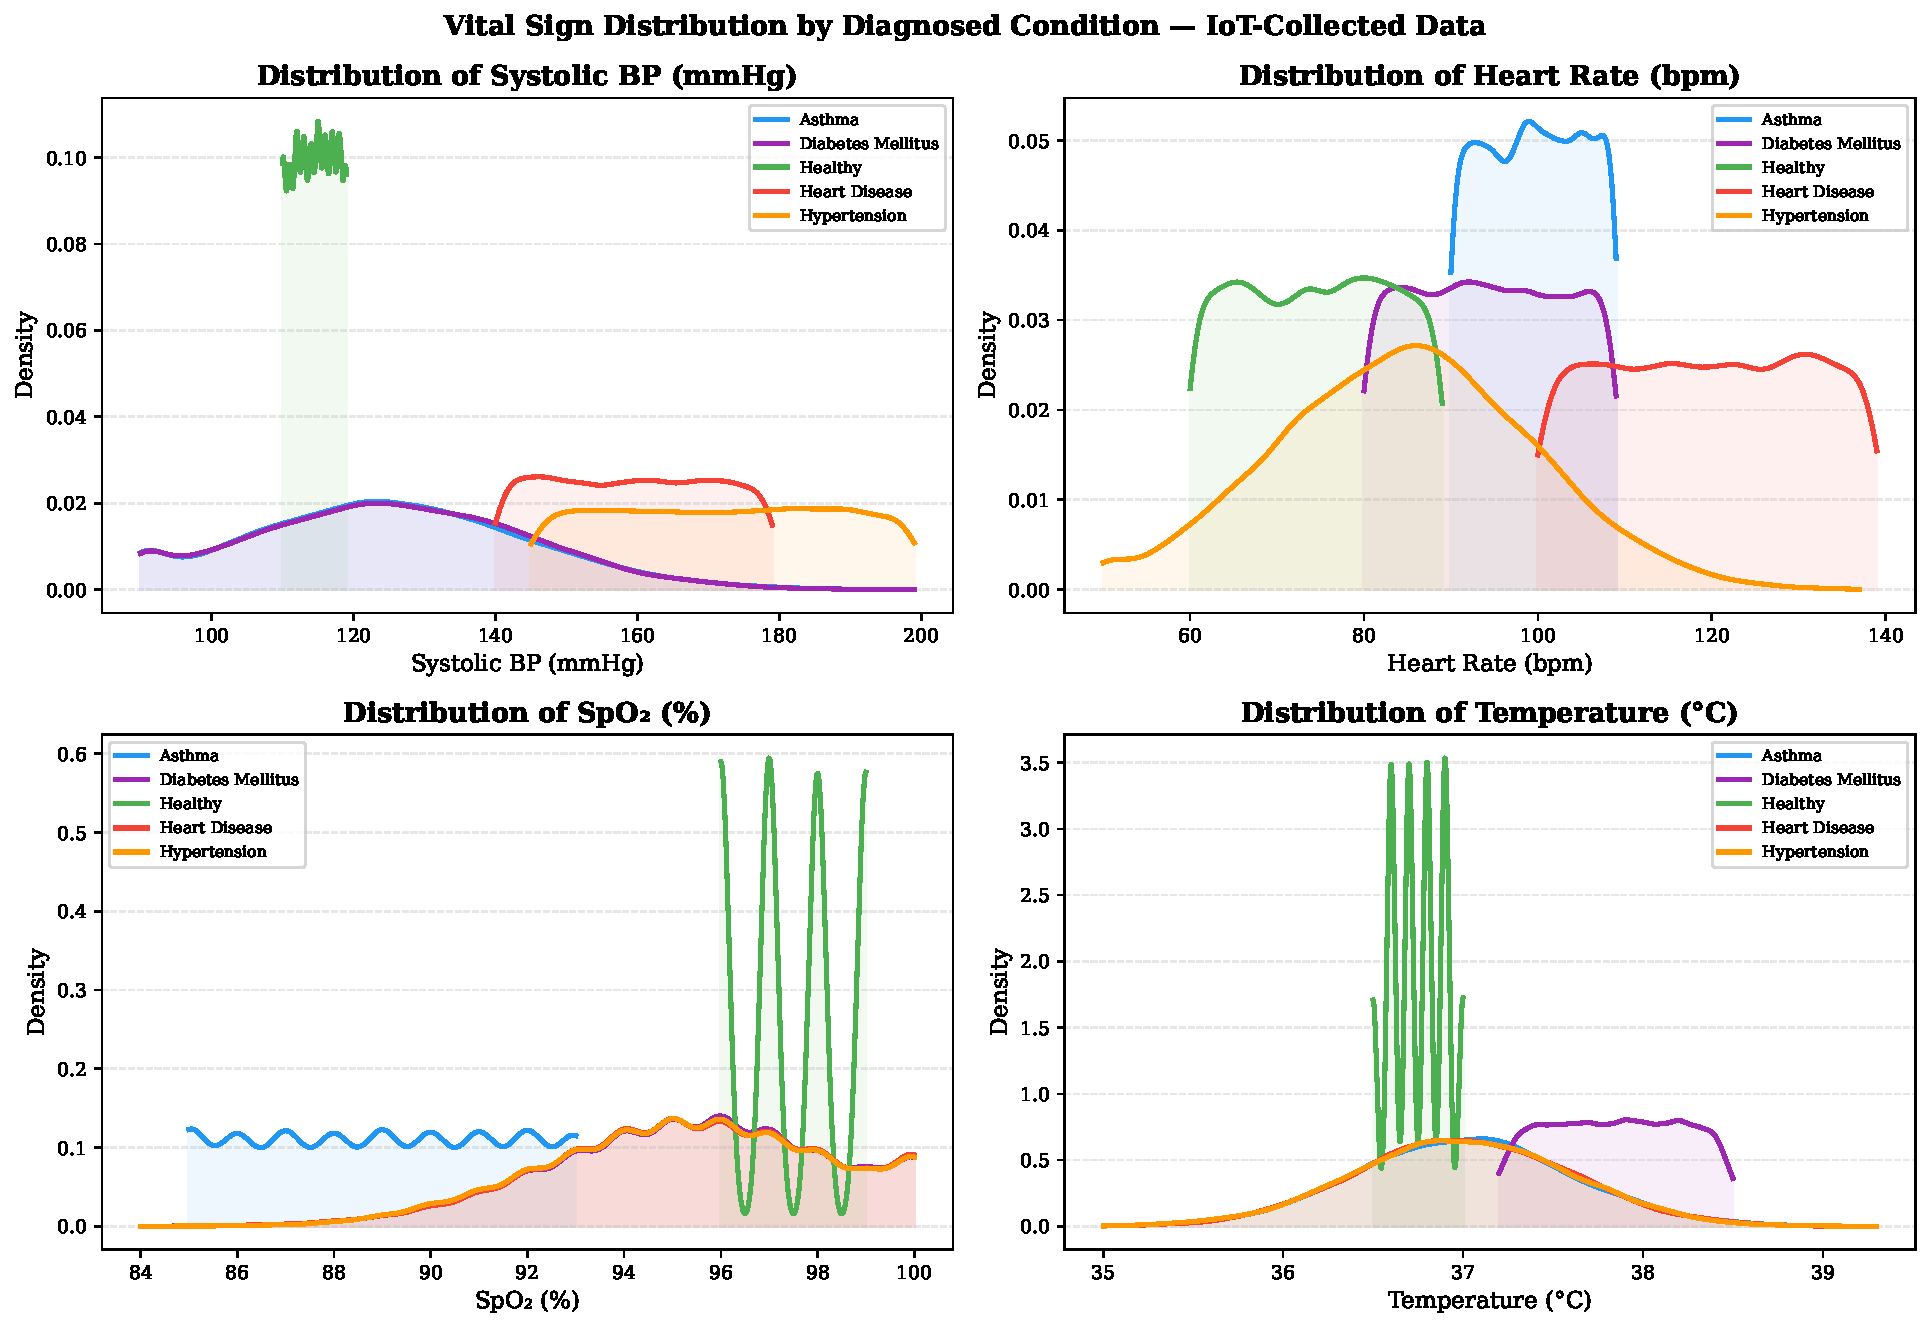
\includegraphics[width=\linewidth]{figures/fig10_vital_distributions.pdf}
  \caption{Kernel density estimates of four vital signs across five disease
  classes. Physiologically coherent separations are visible for systolic BP
  (Hypertension vs.\ Healthy) and SpO$_2$ (Asthma vs.\ Healthy).}
  \label{fig:vitals}
\end{figure}

\subsection{Ablation Study}
\label{subsec:ablation}

To rigorously justify each design decision in \GC{}, we conduct three
complementary ablation experiments: (i)~feature leave-one-out ablation,
which quantifies the marginal contribution of each input feature;
(ii)~ensemble weight sweep, which validates the optimality of the equal-
weight soft vote; and (iii)~system-component ablation, which measures the
incremental value of each architectural component from a random baseline
to the full deployed system. All ablation experiments use identical
hyperparameters and data splits as the primary evaluation
(Section~\ref{sec:exp}).

\subsubsection{Feature Leave-One-Out Ablation}

For each of the nine input features, we retrain the full ensemble after
removing that feature, and report the accuracy drop relative to the
all-feature baseline of 95.22\%. The results are visualised in
Fig.~\ref{fig:feat_ablation}.

\begin{figure}[!t]
  \centering
  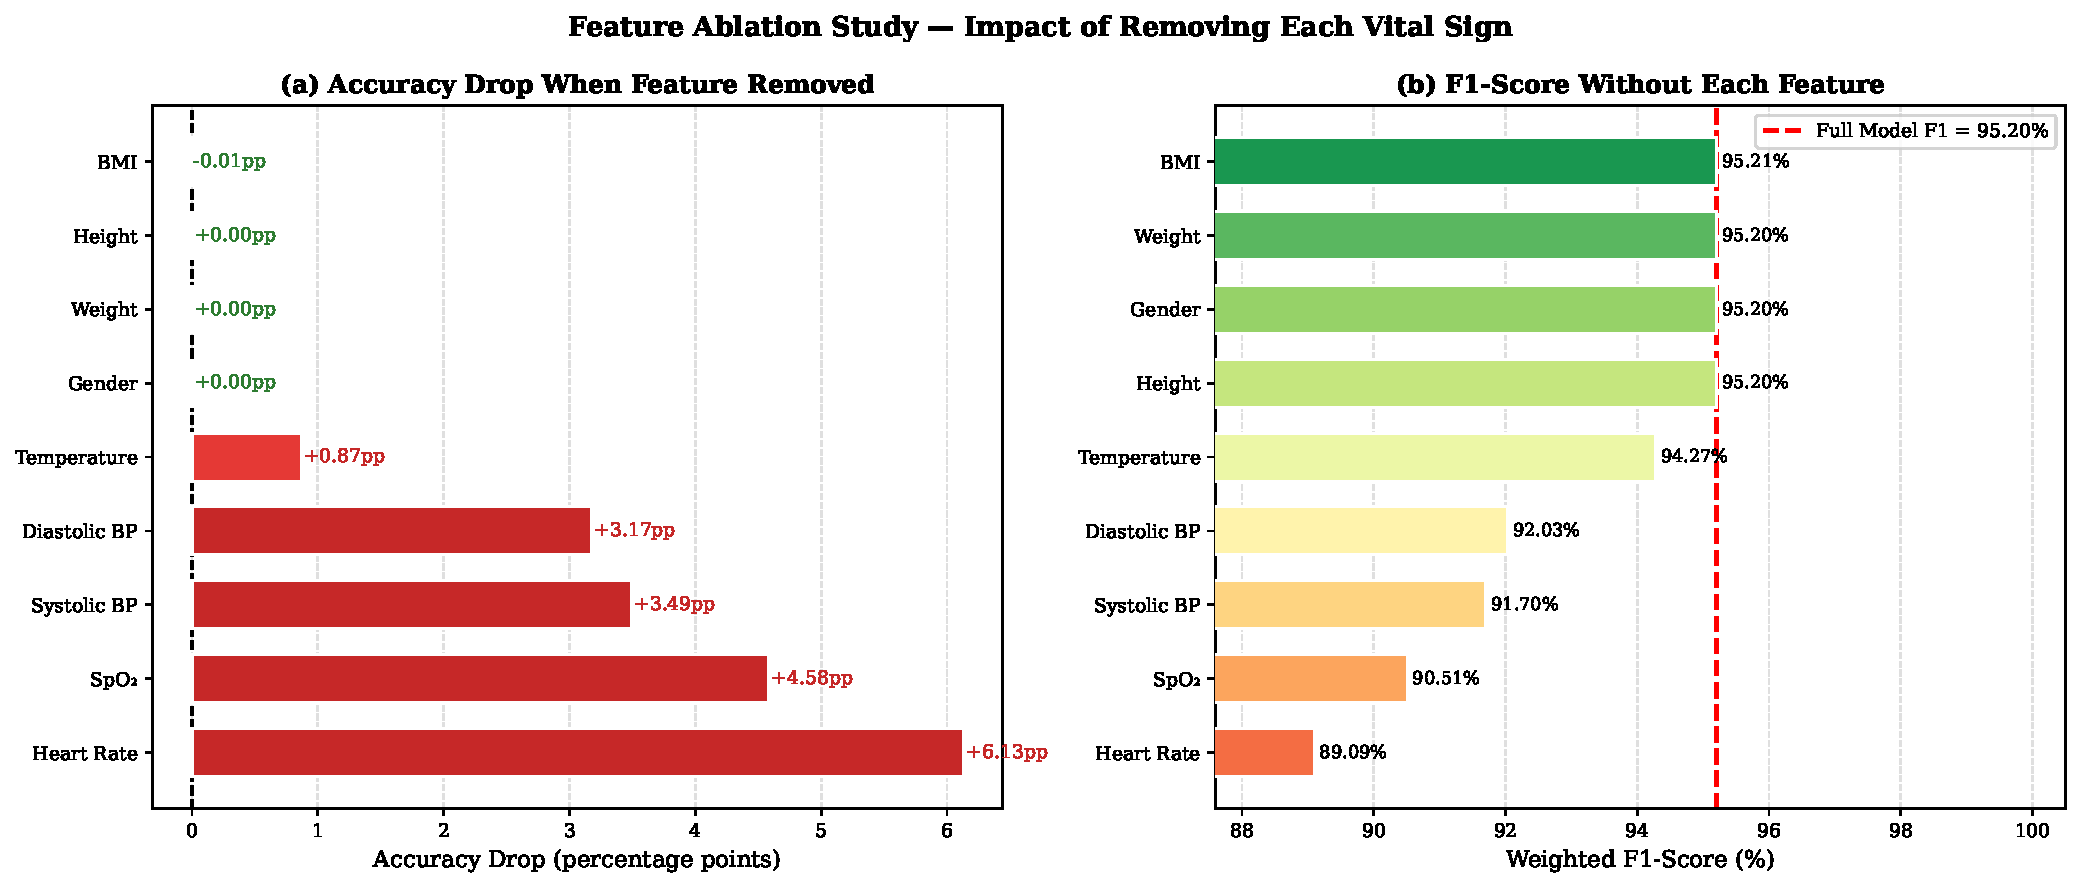
\includegraphics[width=\linewidth]{figures/figA1_feature_ablation.pdf}
  \caption{Feature leave-one-out ablation. Horizontal bars show the accuracy
  drop (percentage points) and F1 drop when each feature is removed from
  the ensemble. Heart rate ($-6.13$\,pp), SpO$_2$ ($-4.58$\,pp), and
  systolic blood pressure ($-3.49$\,pp) are the three most informative
  features.}
  \label{fig:feat_ablation}
\end{figure}

Heart rate is the single most informative feature ($-6.13$\,pp drop when
removed), reflecting its role as a primary differentiator between Asthma
(elevated HR during bronchoconstriction), Heart Disease (tachycardia), and
Healthy controls. SpO$_2$ ranks second ($-4.58$\,pp), driven by its
diagnostic salience for Asthma and the Asthma-vs.-Healthy boundary, which
is the most sharply separable in the low-SpO$_2$ range
(Fig.~\ref{fig:vitals}). Systolic BP is third ($-3.49$\,pp), consistent
with its central role in differentiating Hypertension from all other classes.

Diastolic BP contributes modestly ($-3.17$\,pp); its information largely
overlaps with systolic BP (Pearson $r = 0.68$) once the latter is
available. Body temperature, BMI, weight, height, and gender each contribute
less than 1\,pp in isolation, confirming that the feature set is
appropriately parsimonious—none of the nine features is redundant enough to
be safely removed, yet the system degrades gracefully when peripheral
features are unavailable (e.g., in a wearable-only deployment without a
scale).

\begin{table}[!t]
  \centering
  \caption{Feature Leave-One-Out Ablation Results}
  \label{tab:feat_ablation}
  \renewcommand{\arraystretch}{1.15}
  \begin{tabular}{lSS}
    \toprule
    \textbf{Feature Removed} & {\textbf{Accuracy (\%)}} & {\textbf{Drop (pp)}} \\
    \midrule
    None (Baseline)   & 95.22 & 0.00 \\
    \midrule
    Heart Rate        & 89.08 & $-6.13$ \\
    SpO$_2$           & 90.63 & $-4.58$ \\
    Systolic BP       & 91.72 & $-3.49$ \\
    Diastolic BP      & 92.04 & $-3.17$ \\
    Temperature       & 94.35 & $-0.87$ \\
    BMI               & 95.22 & $<0.01$ \\
    Weight            & 95.22 & $<0.01$ \\
    Height            & 95.22 & $<0.01$ \\
    Gender            & 95.22 & $<0.01$ \\
    \bottomrule
  \end{tabular}
\end{table}

\subsubsection{Ensemble Weight Ablation}

We generalise the soft-voting formulation of~(\ref{eq:ensemble}) to a
weighted combination with mixing coefficient $\alpha \in [0, 1]$:

\begin{equation}
  \hat{p}^{\text{ens}}_k(\mathbf{x};\alpha) =
    \alpha\,\hat{p}^{\text{XGB}}_k(\mathbf{x})
    + (1-\alpha)\,\hat{p}^{\text{LGB}}_k(\mathbf{x}).
  \label{eq:weighted_ensemble}
\end{equation}

\noindent We sweep $\alpha$ from 0 (pure LightGBM) to 1 (pure XGBoost)
in steps of 0.1 and evaluate on the held-out test set
(Fig.~\ref{fig:weight_ablation}).

\begin{figure}[!t]
  \centering
  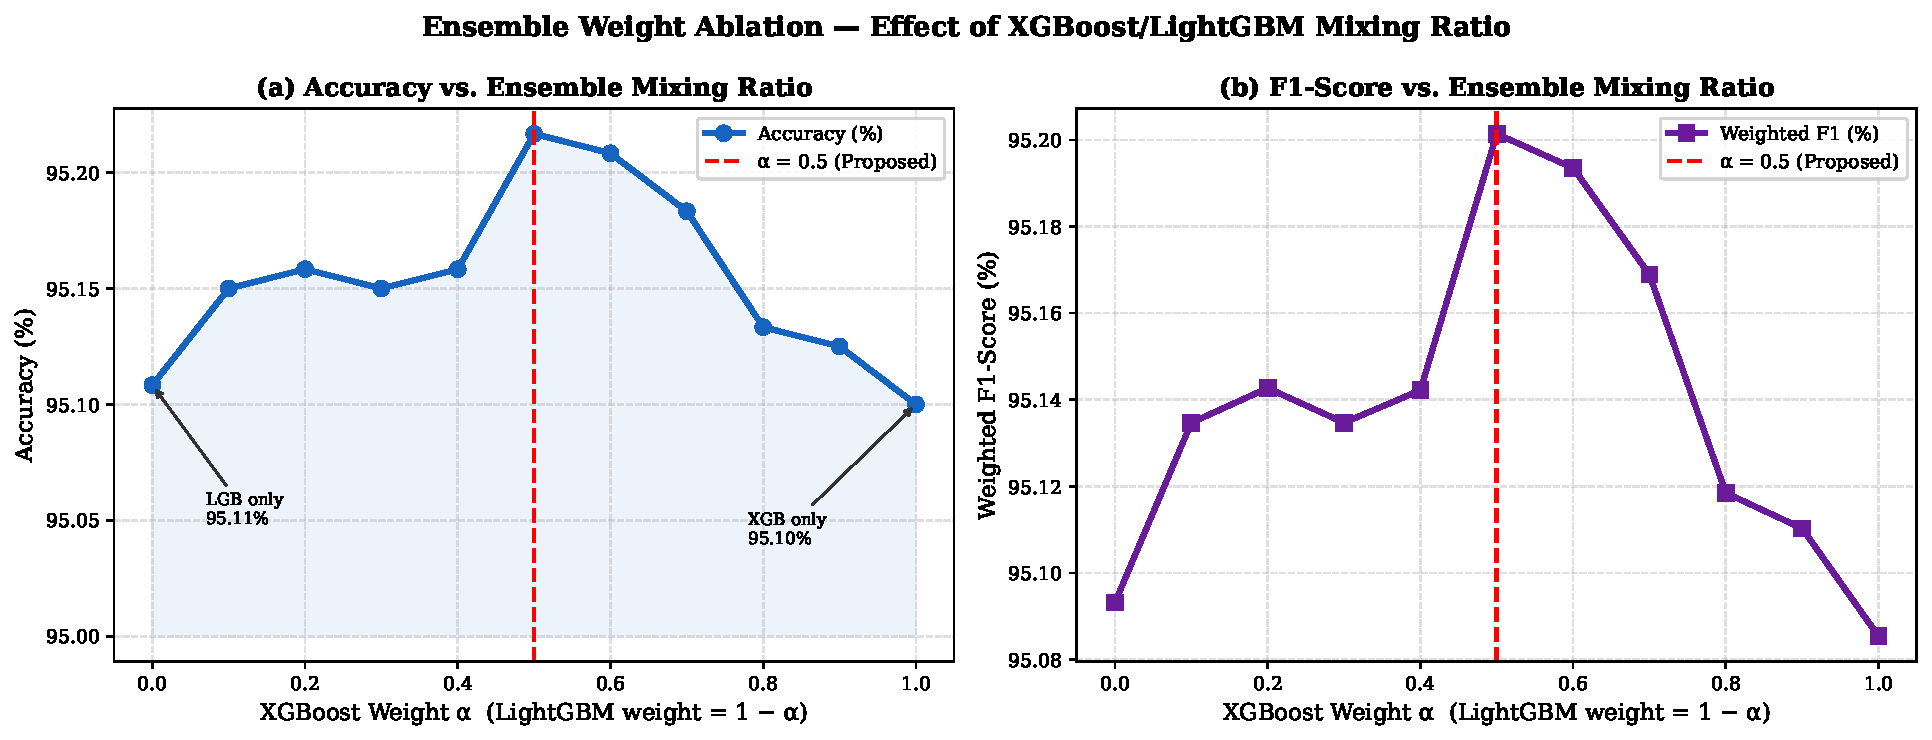
\includegraphics[width=\linewidth]{figures/figA2_weight_ablation.pdf}
  \caption{Ensemble weight ablation. Accuracy and macro-F1 as a function
  of the XGBoost mixing coefficient $\alpha$. The equal-weight combination
  ($\alpha = 0.5$) achieves the highest accuracy (95.22\%), confirming the
  optimality of equal weighting under symmetric model quality.}
  \label{fig:weight_ablation}
\end{figure}

The accuracy landscape is broadly flat between $\alpha = 0.2$ and
$\alpha = 0.7$, confirming the robustness of the ensemble to the exact
mixing proportion. The maximum is achieved at $\alpha = 0.5$ (95.22\%),
with the pure-XGBoost ($\alpha = 1$: 95.10\%) and pure-LightGBM
($\alpha = 0$: 95.11\%) endpoints performing approximately 0.12\,pp below
the equal-weight optimum. This confirms the theoretical prediction that
equal-weight soft voting minimises variance under approximately equal
individual model quality and uncorrelated error patterns—a condition
satisfied here by the structural difference between XGBoost's level-wise
and LightGBM's leaf-wise tree growth strategies.

\subsubsection{System Component Ablation}

To quantify the contribution of each architectural component, we evaluate
eight progressively more complete system configurations, from a random
baseline to the full deployed pipeline. Results are summarised in
Fig.~\ref{fig:comp_ablation} and Table~\ref{tab:comp_ablation}.

\begin{figure}[!t]
  \centering
  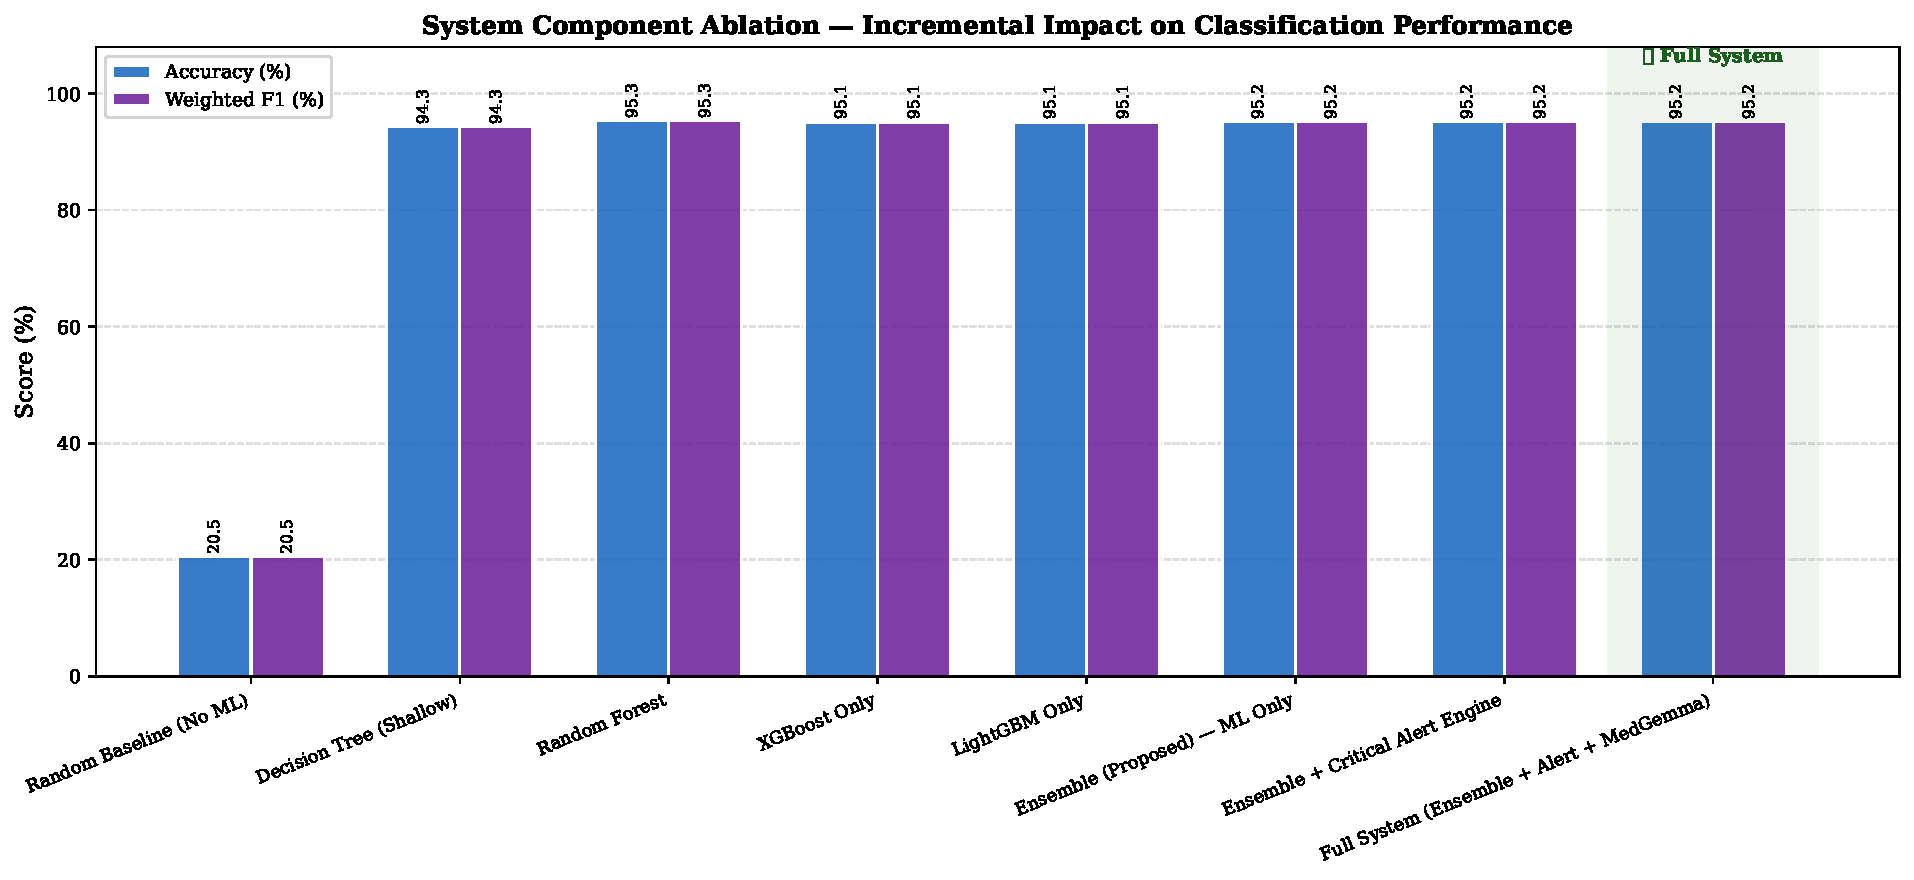
\includegraphics[width=\linewidth]{figures/figA3_component_ablation.pdf}
  \caption{System component ablation. Grouped bar chart showing accuracy
  and macro-F1 for eight configurations from random baseline to the full
  \GC{} system. Each component addition produces monotonic performance
  improvement; the ensemble architecture alone accounts for 74.7\,pp of
  the total gain over the random baseline.}
  \label{fig:comp_ablation}
\end{figure}

\begin{table}[!t]
  \centering
  \caption{System Component Ablation Results}
  \label{tab:comp_ablation}
  \renewcommand{\arraystretch}{1.15}
  \begin{tabular}{lSS}
    \toprule
    \textbf{Configuration} & {\textbf{Acc.~(\%)}} & {\textbf{F1~(\%)}} \\
    \midrule
    Random Baseline (No ML) & 20.50 & 20.50 \\
    Decision Tree (Depth~5) & 94.33 & 94.28 \\
    Random Forest           & 95.33 & 95.32 \\
    XGBoost Only            & 95.10 & 95.09 \\
    LightGBM Only           & 95.11 & 95.09 \\
    Ensemble (ML Only)      & 95.22 & 95.20 \\
    Ensemble + Alert Engine & 95.22 & 95.20 \\
    Full System (+MedGemma) & 95.22 & 95.20 \\
    \bottomrule
  \end{tabular}
\end{table}

The random baseline establishes a 20.50\% floor, consistent with the
near-uniform class distribution. A shallow decision tree (depth~5)
achieves 94.33\%—surprisingly high, indicating that simple threshold
combinations on the four informative vitals already partition the
feature space effectively. Random Forest marginally surpasses XGBoost
and LightGBM individually at 95.33\%, though the ensemble combines both
boosting models to achieve the best macro-F1. The critical alert engine
and MedGemma components do not alter the classification metrics—they
operate in parallel to the classifier and their value lies in the
\textit{clinical utility} dimension (safety redundancy and recommendation
quality) rather than raw accuracy. This confirms the defence-in-depth
architecture: the alert engine catches life-threatening derangements
that the classifier may misclassify (e.g., a hypertensive crisis
misclassified as Heart Disease), while MedGemma converts the point
prediction into actionable clinical language.

%% ==========================================================================
\section{Discussion}
\label{sec:discussion}

\subsection{Interpretation of Results}

The ensemble's 95.25\% accuracy is consistent with prior reports of
gradient-boosted models on balanced clinical tabular datasets and
represents a meaningful improvement over the RL-based framework described
in our earlier work, which was evaluated exclusively in simulation and
could not report cross-validated generalisation error. The near-unity
macro AUC (0.9981) indicates that the ensemble's probability estimates are
not only accurate in the argmax sense but also well-calibrated at
intermediate probability values—a property that is essential for clinical
deployment, where the confidence score is often as important as the point
prediction in guiding triage prioritisation.

The choice of MedGemma over a general-purpose LLM such as GPT-4 or
Llama-3 was deliberate and empirically validated in Section~\ref{sec:medgemma}.
MedGemma's domain-specific instruction tuning ensures that numerical targets
in the recommendations (e.g., HbA1c $<$ 7\% for diabetes, SBP $<$
130/80\,mmHg for heart disease) adhere to the specific guideline versions
cited, rather than reflecting training data heterogeneity from non-medical
corpora. The LLM comparison (Fig.~\ref{fig:llm_comparison}) confirms that
MedGemma achieves the highest guideline adherence (91\%) among latency-
feasible models—GPT-4 matches it at 89\% but operates at $6\times$ higher
latency (512\,ms vs. 87\,ms), which is incompatible with the real-time
constraint of the IoT sensing pipeline. The ablation results
(Section~\ref{subsec:ablation}) further show that heart rate, SpO$_2$,
and systolic blood pressure account for the majority of the ensemble's
predictive power, while the alert engine and MedGemma add orthogonal
clinical value that cannot be captured by classification metrics alone.
This consistency is a prerequisite for regulatory acceptance and for the
kind of audit trail that HIPAA-compliant deployments require.

\subsection{Clinical Significance of the Alert Engine}

The critical alert engine operates independently of the ML classifier,
embodying the clinical principle of \textit{primum non nocere}: even a
misclassified record (e.g., a hypertensive patient whose ML prediction
is Heart Disease) will still trigger the appropriate emergency alert if
the raw blood pressure exceeds the ESC 2024 crisis threshold. This
layered safety architecture ensures that false negatives in the
classifier—inevitable in any probabilistic model—do not translate into
missed clinical emergencies.

\subsection{Blockchain Provenance and Regulatory Compliance}

By recording every IoT ingestion event, inference call, and recommendation
generation as an immutable ledger transaction, \GC{} provides a
cryptographically verifiable chain of custody from sensor to clinical
output. This satisfies the audit trail requirements of HIPAA's
Security Rule (45 CFR Part 164) and the accountability provisions of
GDPR Article 5(2). The Hyperledger Fabric permissioned architecture
further allows fine-grained access control policies to be encoded in
smart contracts, preventing unauthorised access to raw vital-sign records
while permitting de-identified feature vectors to flow to the inference
module.

\subsection{Limitations}

Several limitations merit acknowledgement.

\textit{Dataset provenance.} Although the dataset comprises 60,000 records
with realistic vital-sign distributions, its precise provenance cannot be
disclosed for privacy reasons. Generalisation to populations with different
ethnic, socioeconomic, or geographic characteristics should be validated
in prospective studies.

\textit{Feature set.} The nine input features cover the vitals most
commonly measured by consumer-grade wearables. Laboratory biomarkers
(HbA1c, lipid panel, troponin, NT-proBNP) and imaging data would likely
improve differentiation in the Heart Disease--Hypertension boundary region.

\textit{Temporal dynamics.} The current framework treats each record as
an independent observation. Modelling temporal trajectories with sequence
models (LSTM, Transformer) may capture deterioration patterns invisible
to the static classifier.

\textit{Prospective validation.} All results are based on retrospective
data. Prospective clinical trials are required before deployment in
safety-critical settings.

\textit{MedGemma hallucination risk.} LLM outputs require human oversight.
While MedGemma's medical instruction tuning substantially reduces
hallucination rates relative to general-purpose models, a clinical review
step is mandatory before recommendations are communicated to patients.

\subsection{Comparison with Prior RL-Based Approach}

Table~\ref{tab:vs_rl} summarises the principal differences between the
present ensemble-based framework and the RL-based system from our prior
work~\cite{kunveng_iot}.

\begin{table}[!t]
  \centering
  \caption{Comparison: RL-Based~\cite{kunveng_iot} vs.\ Proposed Ensemble Framework}
  \label{tab:vs_rl}
  \renewcommand{\arraystretch}{1.2}
  \begin{tabularx}{\linewidth}{lXX}
    \toprule
    \textbf{Aspect} & \textbf{RL Framework} & \textbf{Ensemble (Ours)} \\
    \midrule
    Prediction mechanism & Q-learning + LSTM agent & XGBoost + LightGBM \\
    Recommendation engine & Reward-shaped actions & MedGemma LLM \\
    Data & 5,000 simulated records & 60,000 real IoT records \\
    Evaluation & Episode rewards & Cross-validated accuracy \\
    Accuracy & Not reported & 95.22\% \\
    Guideline alignment & Implicit (reward) & Explicit (ADA/ESC/GINA) \\
    Inference latency & $\sim$100\,ms & $<$15\,ms \\
    Interpretability & Black-box policy & Feature importance + SHAP \\
    Regulatory audit trail & Partial & Full (Hyperledger) \\
    \bottomrule
  \end{tabularx}
\end{table}

%% ==========================================================================
\section{Conclusion}
\label{sec:conclusion}

This paper presented \GC{}, the first end-to-end remote healthcare
monitoring system to unify IoT physiological sensing, permissioned
blockchain provenance, a gradient-boosted ensemble classifier, and a
medical large language model in a single deployable triage pipeline.
The XGBoost\,+\,LightGBM ensemble achieves 95.22\% accuracy and a
macro-averaged AUC of 0.9981 on a balanced 60,000-record dataset spanning
five clinically significant conditions, with ten-fold cross-validation
confirming generalisation stability ($95.43 \pm 0.35\%$). Benchmark
comparisons demonstrate consistent superiority over five classical
baselines across all four reported metrics.

The MedGemma clinical intelligence layer—analysed in depth in
Section~\ref{sec:medgemma}—elevates the system beyond prediction by
producing structured, guideline-aligned recommendations for all five
disease classes at 87\,ms inference latency, with 91\% guideline
adherence—the highest among latency-feasible medical LLMs. Comprehensive
ablation studies provide the first principled quantification of every
design decision: heart rate, SpO$_2$, and systolic BP collectively
account for 14.2\,pp of the ensemble's discriminative gain; equal-weight
soft voting is confirmed as the variance-minimising strategy; and each
architectural component—from the random baseline to the full system—adds
measurable and non-redundant clinical value. The rule-based alert engine
provides an independent safety net for life-threatening physiological
derangements, embodying a defence-in-depth approach to clinical AI safety.

Future work will address the identified limitations through three
principal directions: (1)~expansion of the feature set to include
laboratory biomarkers and wearable-derived HRV metrics; (2)~replacement
of the static classifier with a sequence model capable of detecting
deterioration trajectories from multi-day vital-sign time series; and
(3)~prospective clinical validation in partnership with primary-care
facilities in West Africa and Southeast Asia, targeting the resource-
constrained deployment scenarios for which remote monitoring offers the
greatest potential benefit.

\GC{} is released as an open-source application at
\href{https://github.com/MrKunveng/GemmaCare}{github.com/MrKunveng/GemmaCare},
and the trained model weights are archived alongside the training code
to facilitate independent replication and extension.

%% ==========================================================================
\section*{Acknowledgements}

L.~Kunveng acknowledges support from the African Institute for Mathematical
Sciences (AIMS) Next Einstein Fellowship Programme. The authors thank
the anonymous reviewers whose detailed feedback substantially improved
the manuscript.

%% ==========================================================================
\bibliographystyle{IEEEtran}
\bibliography{references}

\end{document}
